% \documentclass[letterpaper,10pt,onecolumn,journal,final]{IEEEtran}
\linespread{2}
% \documentclass[letterpaper,10pt,twocolumn,journal,final]{IEEEtran}
\documentclass[letterpaper,10pt,conference,twocolumn]{IEEEtran}
% \documentclass[a4paper,10pt,onecolumn]{IEEEtran}
% \documentclass[a4paper, 10pt, conference]{ieeeconf}
%\documentclass[draft,a4paper,10pt,onecolumn]{ieeeconf}

\IEEEoverridecommandlockouts

\usepackage[active]{srcltx}

\usepackage{epsfig}
\usepackage{amsmath}
%\usepackage{amsthm}
\usepackage{amssymb}
\usepackage{psfrag}
\usepackage[T1]{fontenc}
\usepackage{graphicx}
\usepackage{txfonts}

\bibliographystyle{IEEEtran}

\graphicspath{{../figure/}}

\newtheorem{dfn}{Definition}
% \newtheorem{not}[]{Notation}
\newtheorem{thm}{Theorem}[section]
\newtheorem{lem}[thm]{Lemma}
\newtheorem{cor}[thm]{Corollary}
\newtheorem{obs}{Observation}
% \newtheorem{definition}{Definition}

\newcommand{\sat}{\mathrm{sat}}
\newcommand{\eps}{\epsilon}
\newcommand{\csi}{\xi}
\newcommand{\sect}{\mathrm{sect}}
\newcommand{\sgn}{\mathrm{sgn}}
\newcommand{\w}{\omega}
\newcommand{\Csi}{\Xi}
\newcommand{\Real}{\mathbb{R}}
\newcommand{\Nat}{\mathbb{N}}
\newcommand{\ellips}{\mathcal{E}}

\title{Less conservative absolute stability criteria using Integral Quadratic Constraints}
% \author{}
\author{
	Donatello Materassi\IEEEauthorrefmark{1} and
	Murti V.~Salapaka\IEEEauthorrefmark{7} \medskip\\
		Department of Electrical and Computer Engineering,\\
		University of Minnesota,\\
		200 Union St SE, 55455, Minneapolis (MN) \\
	\IEEEauthorrefmark{1}
		{\tt\small mater013@umn.edu} \medskip \qquad
	\IEEEauthorrefmark{7}
		{\tt\small murtis@umn.edu}
}

\begin{document}

\maketitle
\thispagestyle{empty}
\pagestyle{empty}

\begin{abstract}
Lur'e systems, that are described by the feedback interconnection of a linear time invariant system and a nonlinear system, form an important class of nonlinear systems arising in many modern applications. A number of absolute stability criteria are available where the stability is guaranteed with the nonlinearity restricted to a pre-specified set.
Most of these criteria provide sufficient conditions for absolute stability, thus  lessening the conservativeness remains a challenge.
A method of reducing conservativeness is to first estimate the part of the nonlinearity that is appropriate from an asymptotic sense followed by the application of  a preferred absolute stability criteria to the more restricted nonlinearity. A comprehensive  framework that incorporates the above approach is developed in this paper that employs a methodology based on Integral Quadratic Constraints as a means of  describing  the nonlinearity.
It is shown that the developed framework can be used to conclude absolute stability of Lur'e interconnections where all of the existing criteria fail to be satisfied. Indeed, examples are provided where the nonlinearity does not fall into the classes assumed by existing absolute criteria. Another contribution of the article is the extension of IQC theory.
\end{abstract}

\section{Introduction}
In this work, we focus on an important class of nonlinear models given by the feedback interconnection of a linear time-invariant system $\mathcal{G}$ with a nonlinear block $\mathcal{N}$ (see Figure~\ref{fig:lur'e}).
\begin{figure}
	\centering
	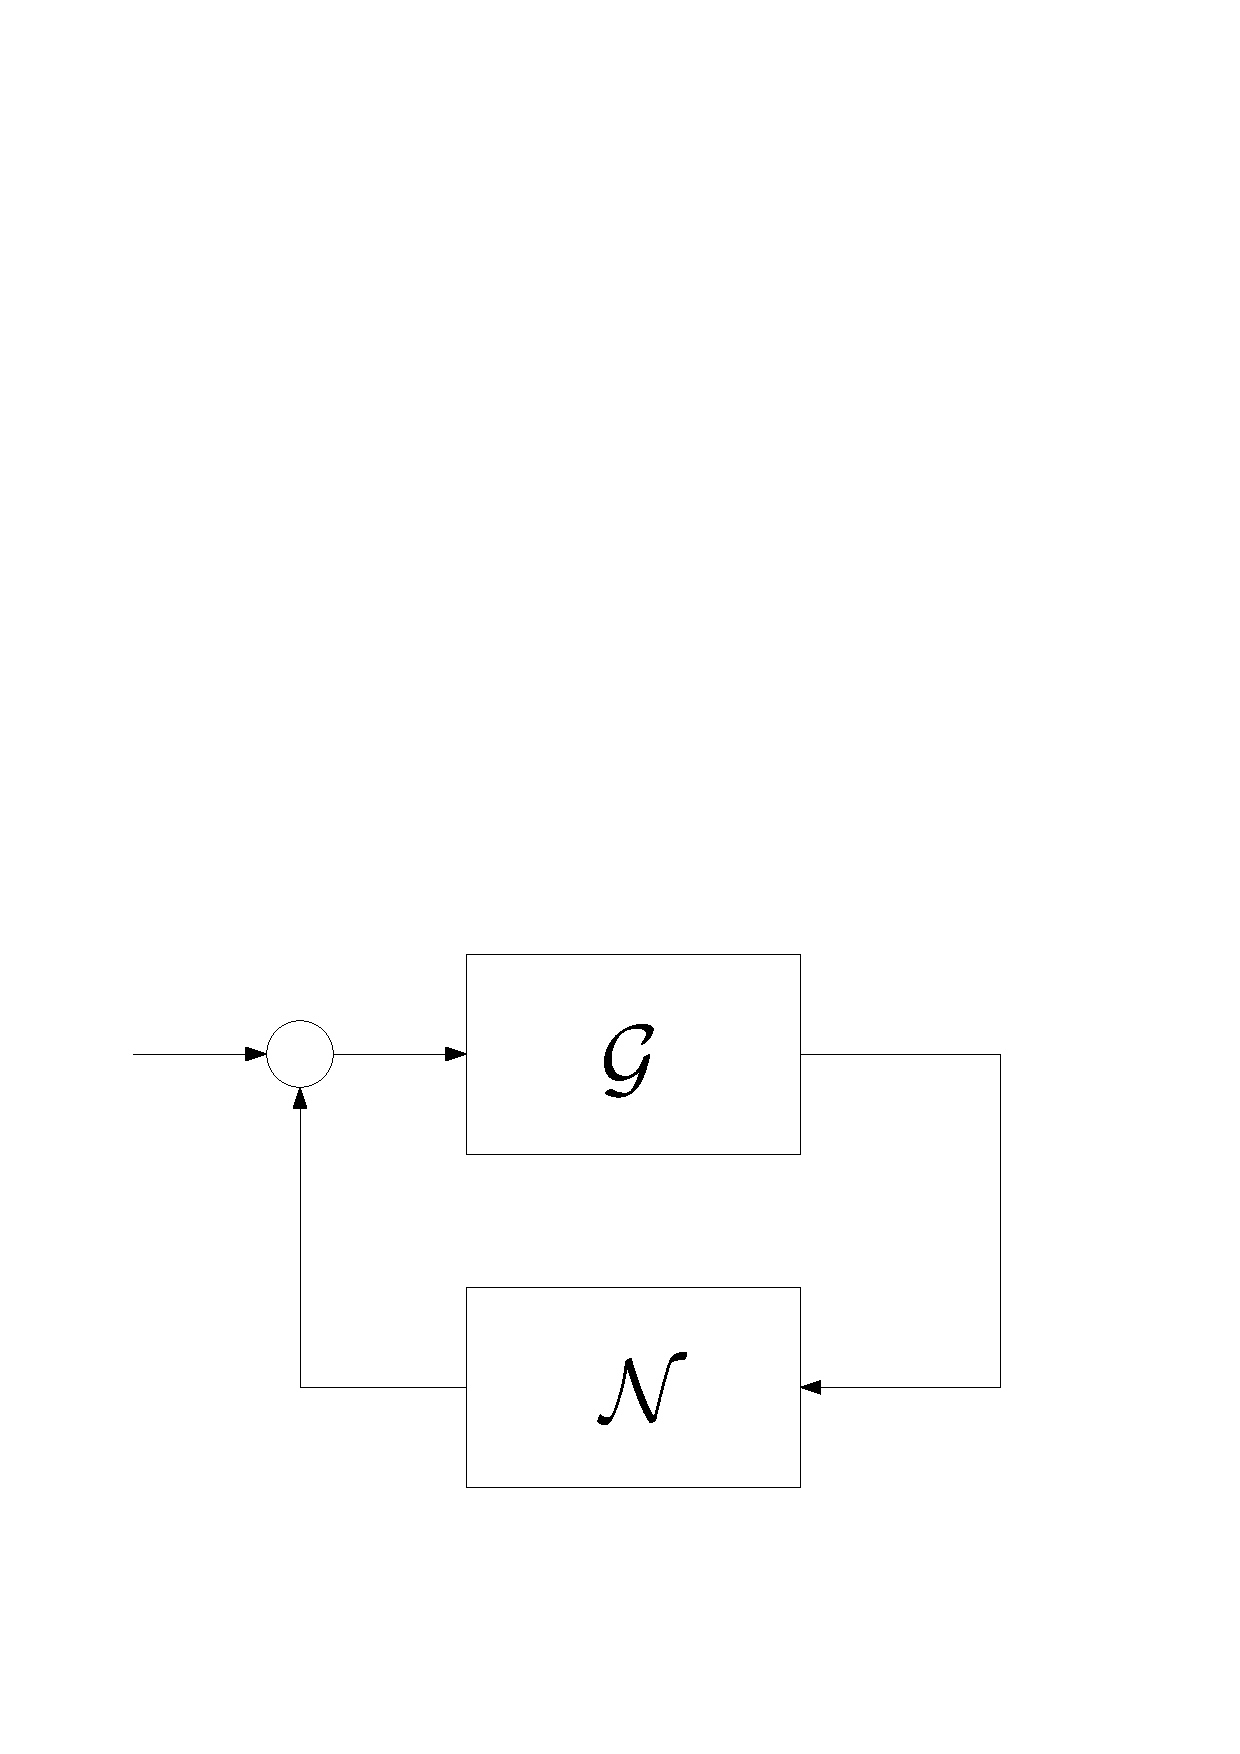
\includegraphics[width=0.75\columnwidth]{lure}
	\caption{A Lur'e System\label{fig:lur'e}}
\end{figure}
Models of this kind are known in the literature as Lur'e systems \cite{LurPos44} and a large number of real systems have this structure. Recent examples are provided by Atomic Force Microscopes \cite{SebSal01},\cite{SebGan05} and other Microelectromechanical systems \cite{WieSeb05}, \cite{SebWie08}, \cite{AgaSah08}.
Many studies targeted the problem of ``absolute stability'',  where the  stability is sought with respect to  an entire class, and thus the related  results provide a robust notion of stability.  
Classical results include the Popov (see \cite{Pop62}) and the circle criteria (see \cite{San64} and \cite{Zam66b}) that provide sufficient conditions for global asymptotic stability  when the nonlinearity is restricted to be  time-invariant and time varying respectively.
% For a recent survey of absolute stability results see \cite{Lib06}. 
% Most existing approaches of ascertaining absolute stability involve a realization of the linear part of the Lur'e model and a Lyapunov function whose derivative along the trajectories of the interconnection dynamics is shown to be negative with the nonlinearity restricted to a targeted class (see \cite{NarTay73}).
% For example, in the  circle criterion  the  input-output characteristic of the linear part being positive-real is employed to obtain a Lyapunov function using the Kalman-Yakubovich-Popov lemma (\cite{Khalil,Ran96})  whose derivative along the possible  state trajectories is shown  to be negative to conclude absolute stability. There are input-output ways of defining and ascertaining absolute stability without taking recourse to a state-space realization or a Lyapunov function, (see for example, the derivation of the circle and Popov criteria in \cite{Vidyasagar}). 
A relatively new approach
% involving only input-output maps
is given by the Integral Quadratic Constraint (IQC) methods pioneered in \cite{MegRan97}. In this approach, a quadratic constraint is used to characterize the nonlinearity playing the role of the sector condition used in classical absolute stability criteria. A challenge of the existing results is the possible conservativeness as the results  provide only sufficient conditions. Thus it is possible that the nonlinearity does not satisfy the absolute stability criteria with the Lur'e interconnection being stable. Also, often it is possible that the nonlinearity does not fall under the standard sector conditions being assumed by many of  absolute stability criteria and thus are inapplicable to the nonlinearity in question. Here too, the IQC framework provides a more general approach of describing the nonlinearity. Furthermore, since the prior sector conditions can be derived using the IQC approach, the IQC approach provides a powerful unifying theoretical framework.
% The ability of seamlessly integrating different IQC characterizations of the nonlinearity is another powerful feature of the IQC approach.

% Recent results related to Lur'e systems include the estimation of attraction domains \cite{HuxHua04,MarAlb06}, conditions for absolute stability and for the existence of periodic orbits \cite{WulSho07} and stability analysis when nonlinear operator has slope constraints \cite{LeePar07}.
% The conservativeness of various absolute stability criteria is still an open issue \cite{BloSon99} and deriving weaker conditions for absolute stability can lead to a greater applicability.

In all the absolute stability approaches, the conditions on the linear and on the nonlinear parts are imposed separately. A closer coupling can be brought about by first estimating which is the important part of the phase space where the trajectory reside thereby limiting the real extent of the nonlinear regime being explored. This opens up a new way of reducing the conservativeness of the conditions for absolute stability.
Indeed, it is possible that the nonlinearity admits a characterization, for example a sector condition, that is severe enough for the absolute stability result not to hold. However, it is possible that the nonlinearity that is eventually explored lies only in a restricted tractable region, for which standard tools of analysis can be employed.
The above observation forms the central concept developed in the paper where a bounded region where the nonlinearity is eventually explored is estimated and then a preferred absolute stability criterion is applied to the restricted nonlinearity.
We accomplish the estimate of the bounded region by extending Integral Quadratic Constraint techniques to analyze practical stability properties of the system. 
Similar concepts are suggested in \cite{Meg95} even though in a different context.
Adequate machinery is developed to follow a time-domain analysis based on Lyapunov functions.
In section \ref{sec:problemdefinition} the problem of absolute stability is defined; in section \ref{sec:BLQC} and in section \ref{sec:BIQC} the IQC framework is extended by the notions of the notion of Biased Local Quadratic Constraint (BLQC) and of Biased Integral Quadratic Constraint (BIQC); in section \ref{sec:static and dynamic BIQC} we show how dynamic BIQC's can be translated to static BIQC's and finally in section \ref{sec:examples} we provide illustrative examples of the presented techniques.

\section{Notation}\label{sec:notation}
In this section we introduce the basic notation we will employ to present our results.
First, we define a generalization of Positively Invariant sets
\begin{dfn}
	Let $\mathcal{S}$ be a dynamical system described by an initial condition problem
	\begin{align}\label{eq:dynsys}
			\dot x = f(t,x), & \qquad x(t_0)=x_0
	\end{align}
	where the uniqueness of solutions is guaranteed. Suppose that the state $x$ of the system assumes values in a normed space $D$ and that $\phi(t,t_0,x_0)$ is the trajectory related to the initial condition $(t_0,x_0)$. We say that $E$ is an eventually positively invariant (EPI) set for $\mathcal{S}$ if and only if, for all $t_0$ and for all $x_0 \in E$, there exists $T\geq t_0$ such that
	\begin{equation}\nonumber
		\phi(t,t_0,x_0) \in E \qquad \text{for all}~t>T.
	\end{equation}
\end{dfn}
\noindent
As is clear from the definition, a trajectory starting from an initial condition $(t_0, x_0)$ in an EPI set $E$ may leave the set, but there exists a time $T$ after which it permanently remains in $E$.
% Note that the time $T$, in general, depends on $(t_0, x_0)$.
We also remind the definition of a global attractor.
\begin{dfn}
	A subset $E$ is a global attractor for the dynamical system (\ref{eq:dynsys}) if and only if, for all $x_0\in D$ and for all $\eps>0$ there exists a time $T=T(\eps,x_0)$ such that, for any $t>T$
	\begin{equation}\nonumber
		\inf_{z\in E}\{\|\phi(t,t_0,x_0) -z \}<\eps.
	\end{equation}
\end{dfn}
\noindent
Since we will deal with quadratic Lyapunov functions in finite dimensional state spaces, a handy notation for elliptical domains follows.
\begin{dfn}
	Let $P$ be a strictly positive $n\times n$ matrix and let $H$ be a real nonnegative value. We define
	\begin{equation}\nonumber
		\ellips_P(H)\coloneqq 
			\left\{ 
				x\in \Real^n : x^T P x \leq H
			\right\}.
	\end{equation}
\end{dfn}
We will also need to decompose a signed function using non-negative functions.
\begin{dfn}
	Let $\gamma(t)$ be a real valued function. We define
	\begin{equation}\nonumber
		\gamma^{(+)}(t)=
			\left\{\begin{array}{ll}
				\gamma(t)\qquad &\text{if } \gamma(t)\geq 0\\
				0 & \text{otherwise}
			\end{array}\right.
	\end{equation}
	and
	\begin{equation}\nonumber
		\gamma^{(-)}(t)=
			\left\{\begin{array}{ll}
				-\gamma(t)\qquad &\text{if } \gamma(t)\leq 0\\
				0 & \text{otherwise}.
			\end{array}\right.
	\end{equation}
\end{dfn}
% \begin{dfn}
% 	Given a transfer matrix $G(s)$ we say that $(A,B,C,D)$ is one of its realizations if and only if
% 	\begin{equation}\nonumber
% 		G(s)=C(sI-A)^{-1}B+D
% 	\end{equation}
% \end{dfn}

Finally, we will denote by $\hat x(\w)$ the Fourier transform of the signal $x(t)$.

\section{Problem definition}\label{sec:problemdefinition}
Let us consider a Lur'e system depicted in Figure~\ref{fig:lur'e}.
Assume that the linear system $\mathcal{G}$ is strictly proper with transfer function $G(s)$ and that the nonlinear block $\mathcal{N}$ can be described by a possibly time-varying operator $\Csi$. 
The differential equation representing such a feedback interconnection is symbolically expressed by
\begin{equation}\label{eq:symlur'e}
	y = G(d/dt)~\Csi(t, y(\cdot))
\end{equation}
where $y$ is the output of the system.
The problem we are considering is to derive conditions on $G(s)$ and $\Csi$ in order to determine the practical or asymptotic stability of the system. In the following sections we examine different kind of quadratic constraints which, if fulfilled by the feedback operator $\Csi$, allow the problem to be addressed via LMI's.

\section{Biased Local Quadratic Constraints}\label{sec:BLQC}
We start our study by considering a strict form of quadratic constraints involving the input and the output of an operator~$\Csi$.
\begin{dfn}
	Given a constant matrix $\Sigma\geq 0$, we define the quadratic form $\sigma: \Real^{p} \times \Real^{m} \rightarrow \Real$
		\begin{equation}\nonumber
			\sigma(y,u)=
					\left(\begin{array}{c}
						y\\
						u
					\end{array}\right)^*
					\Sigma
					\left(\begin{array}{c}
						y\\
						u
					\end{array}\right).
		\end{equation}
	We say that a nonlinearity $\Xi(\cdot)$ satisfies the Biased Local Quadratic Constraint (BLQC) defined by $\sigma$ with bias $M>0$, if and only if
	\begin{equation}\label{eq:defLQC}
		\sigma(y(t),\xi(t)) + M\geq 0 \qquad \text{for all}~t>0
	\end{equation}
	for any signals $y(t),\xi(t)\in L_{2e}$, where $\xi(t)=\Xi(y(t))$.
	If the BLQC is satisfied for all $M>0$, we say that (\ref{eq:defLQC}) is an Unbiased Local Quadratic Constraint (ULQC).
\end{dfn}
\noindent
% \begin{obs}
	Note that many conditions in absolute stability theory are expressed in the form of ULQC's. Consider the standard sector condition for SISO nonlinearities which is employed in the Circle, Popov and many other criteria
	\begin{equation*}
% 		\label{eq:sectorcondition}
		\alpha y^2 \leq y \Xi(y) \leq \beta y^2,
	\end{equation*}
	where $\alpha$ and $\beta$ are the sector bounds. It can be written in the equivalent matrix notation
	%TODO: replace $\Sigma$
	\begin{equation}\nonumber
		0\leq 
		\left(\begin{array}{c}
			y\\
			\Xi
		\end{array}\right)^*
		\Sigma
		\left(\begin{array}{c}
			y\\
			\Xi
		\end{array}\right).
	\end{equation}
	In the $(y,\Xi)$ plane the nonlinearity lies in the region described by the lines $\Xi=\alpha~y$ and $\Xi=\beta~y$. The presence of a bias $M$ allows the nonlinearity to be more ``free'' in the neighborhood of the origin whereas its behaviour remains quite the same when it is far from the origin. Indeed, the relation
	\begin{equation}\nonumber
		0\leq 
		\left(\begin{array}{c}
			y\\
			\Xi
		\end{array}\right)^*
		\Sigma
		\left(\begin{array}{c}
			y\\
			\Xi
		\end{array}\right) +M,
	\end{equation}
in the SISO case, is satisfied by all the nonlinearities lying in a ``hyperbolic sector''.
This scenario is qualitatively depicted in Figure \ref{fig:HyperSector}.
% \end{obs}
\begin{figure}[hbt]
	\begin{center}
% 		\psfrag{y}{$y$}
% 		\psfrag{n(t,y)}{$\Xi(y)$}
		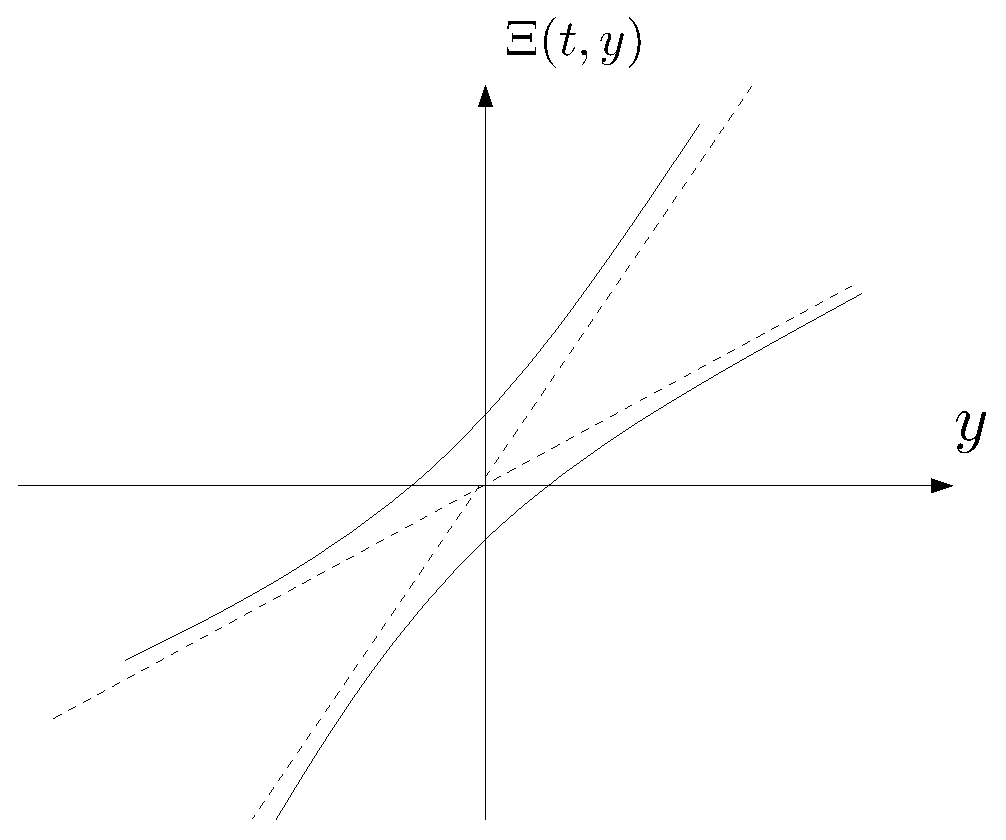
\includegraphics[width=0.7\columnwidth]{hypersector}
	\end{center}
	\caption{A hyperbolic sector\label{fig:HyperSector}}
\end{figure}
We show the following result.
\begin{thm}\label{thm:bottle_blq}
	Let $\mathcal{S}$ be the Lur'e system described by (\ref{eq:symlur'e}). Let $G(s)$ be a strictly proper transfer function and let $(A,B,C,0)$ be
	a minimal realization of $G(s)$ with state $x \in \Real^{n}$.
	Suppose that $\Csi$ satisfies the BLQC given by the quadratic form $\sigma$
	\begin{equation*}
		\sigma(y,\xi)=
			\left(
				\begin{array}{c}
					y \\
					\xi
				\end{array}
			\right)^T
			\Sigma
			\left(
				\begin{array}{c}
					y \\
					\xi
				\end{array}
			\right)
			\geq -M
	\end{equation*}
	with 
	\begin{equation*}
		\Sigma=
		\left(
			\begin{array}{cc}
				Q	& S \\
				S^T	& R
			\end{array}
		\right).
	\end{equation*}
	If there exists a solution $(P, r)$ to the following LMI
	\begin{equation*}
		\left[
			\begin{array}{cc}
				A^TP+PA+C^TQC+rP	& PB+C^TS \\
				B^TP+S^TC		& R
			\end{array}
		\right] < 0
	\end{equation*}
	with $P\in \Real^{n\times n}$, $P=P^T$, $P>0$, $r \in \Real^+$,
	then, for every $H>M/r$, the set $\ellips_P(H)$ is a positively invariant set and a global attractor for $\mathcal{S}$.
\end{thm}
\begin{proof}
	Consider the quadratic function $V(x)=x^TPx$.
	The derivative of $V(t)$ along a trajectory is given by
	\begin{align*}
		dV/dt&=x^TA^TPx+x^TPAx+\xi^T B^T Px + x^T P B\xi=\\
			&=x^TA^TPx+x^TPAx+\xi^T B^T Px + x^T P B\xi+\\
			&\qquad +x^TC^TQCx+2x^TC^TS\xi+\xi^TR\xi-\sigma(y,\xi)\leq\\
			&\leq -r x^TPx -\sigma(y,\xi).
	\end{align*}
	By hypothesis we have that
	\begin{equation}\label{eq:diffVhardIQC}
		dV/dt \leq -r x^TPx +M.
	\end{equation}
	Consider the set $\ellips_P(H)$.\\
	First, we prove that there exists a time $t_1>0$ such that
	$V(x(t_1))<H$ which implies $x(t_1)\in \ellips_P(H)$.\\
	By contradiction, $V(x(t))\geq H$ for all $t>0$.
	Let $\eta$ be such that $0<\eta<H-M/r$.
	Integrating both sides of (\ref{eq:diffVhardIQC}) from $0$ to $t$ yields
	\begin{equation*}
		V(x(t)) \leq V(x(0))-r \int_0^t (x(\tau)^TPx(\tau) +M)d\tau
			\leq V(x(0)) -\eta~t.
	\end{equation*}
	Since $V(t)$ is non negative for all $t$, we obtain a contradiction
	choosing $t>V(x(0))/\eta$.\\
	Now, we prove that $x(t)\in \ellips_P(H)$ for all $t\geq t_1$.
	This is equivalent to say that $t>t_1$ implies $V(x(t))\leq H$.\\
	By contradiction, there exists $t_3>t_1$ such that $V(x(t_3))>H$.
	Consider the set $\mathcal{T}=\{t_1\leq t \leq t_3| V(x(t))\leq H\}$
	and define $t_2=\sup \mathcal{T}$. We have that $t_2\in \mathcal{T}$
	because $V(x(t))$ is continuous. Thus $t_2 \neq t_3$.
	$V$ is also differentiable, thus, for the mean value theorem \cite{Rudin76}, there exists $t^*$ such that $t_2<t^*<t_3$ and
	\begin{equation*}
		0<V(x(t_3))-V(x(t_2))=\frac{dV}{dt}(x(t^*))~[t_3 -t_2],
	\end{equation*}
	which implies $\frac{dV}{dt}(x(t^*))>0$.
	This is a contradiction because we also have $V(x(t^*))>H>M/r$
	which implies $\dot V(x(t^*))<0$.
\end{proof}
\begin{cor}
	If the ULQC is satisfied, then every ellipsoid $\ellips_P(H)$ with $H>0$ is an EPI set for the system trajectories. Thus, we can conclude global asymptotic stability of the system.
\end{cor}
% We stress that these results rely on the existence of a Lyapunov function for the Lur'e system. LMI's are a tool to achieve this objective.
% The same approach can be applied in order to obtain a generalization of the Circle Criterion in Passivity Theory as proposed in \cite{MatSal06} or the Popov Criterion.
% Indeed, the application of the KYP lemma (instead of the numerical solution of an LMI) leads to the definition of a Lyapunov function in both these results.
% In the Appendix we consider these two cases in detail.
% The relaxed condition of BLQC provides an estimate of the positively invariant set.

\section{Biased Integral Quadratic Constraints}\label{sec:BIQC}
BLQC's are relations involving the input and the output of an operator pointwise in time. A Biased Integral Quadratic Constraint (BIQC), defined below, involves the input and the output of an operator on an time interval (usually $[0, +\infty)$).
\begin{dfn}\label{dfn:BIQC}
	A nonlinear function $\Xi$ satisfies the BIQC defined by $\sigma$ with bias $M>0$ if and only if
	\begin{equation}\label{eq:biqc_condition}
		\liminf_{t\rightarrow +\infty}
			\int_0^{~t}[\sigma(y(\tau),\xi(\tau)) + M ]d\tau\geq 0,
	\end{equation}
	where $\xi(t)=\Csi(y(t))$.
	We also use $\Csi \in BIQC(\sigma,M)$, if $\Xi$ satisfies the condition (\ref{eq:biqc_condition}). If $\in BIQC(\sigma,M)$, for all $M>0$, we say that $\Xi$ satisfies the Unbiased Integral Quadratic Constraint (UIQC) and abusing the notation we write $\in BIQC(\sigma,0)$.
\end{dfn}
\begin{obs}
	If a nonlinearity satisfies a BLQC with bias $M$, then it follows that a BIQC is satisfied by the same nonlinearity with the same bias.
\end{obs}
% \begin{obs}
% 	Conversely, note that if the nonlinearity $\Xi(\cdot)$ is static and single-valued, then the BIQC condition is equivalent to the BLQC one.
% \end{obs}
%
% We can interpret the quadratic form $\sigma$ as a correlator filter between the two signals $y(t)$ and $\xi(t)$.
% The following lemma provides an equivalence among a BIQC condition and a condition on the average power of such a filtered correlation.
% \begin{lem}
% 	The following statements are equivalent
% 	\begin{itemize}
% 	\item
% 		\begin{equation}\label{eq:biqcA}
% 			\liminf_{T\rightarrow +\infty}
% 				\int_0^{T}[\sigma(\tau)+M+\eta]d\tau\geq 0
% 				\qquad \text{for all}~\eta>0.
% 		\end{equation}
% 	\item
% 		\begin{equation}\label{eq:biqcB}
% 			\liminf_{T\rightarrow +\infty}\frac{1}{T}
% 			\int_0^{T}[\sigma(\tau)+M]d\tau\geq 0.
% 		\end{equation}
% 	\end{itemize}
% \end{lem}
% \begin{proof}
% 	Let (\ref{eq:biqcA}) be satisfied and supposed $\eta>0$ is fixed.
% 	Then, for every $\eps>0$ there exists $\bar T=\bar T(\eps,\eta)$ such that $T\geq \bar T$ implies that
% 	\begin{equation}\nonumber
% 		\int_0^{T}[\sigma(\tau)+M+\eta]d\tau\geq -\eps.
% 	\end{equation}
% 	Choosing $T>\bar T (\eps/2,\eps/2)$ leads to
% 	\begin{equation}\nonumber
% 		\int_0^{T}[\sigma(\tau)+M+\eps/2]d\tau\geq -\frac{\eps}{2}.
% 	\end{equation}
% 	Define $\hat T(\eps):=\max\{1,\bar T(\eps/2,\eps/2)\}$.
% 	If $T>\hat T(\eps)$, then
% 	\begin{equation}\nonumber
% 		\frac{1}{T}\int_0^{T}[\sigma(\tau)+M]d\tau\geq
% 			-\frac{\eps}{2T}-\frac{\eps}{2}\geq -\eps.
% 	\end{equation}
% 	Thus (\ref{eq:biqcB}) is satisfied.\\
% 	Suppose (\ref{eq:biqcB}) is satisfied and suppose $\eta>0$ is fixed. If $\eps<\eta$, then there exists $\hat T$ such that $T>\hat T$ implies
% 	\begin{equation}\nonumber
% 		\frac{1}{T}\int_0^{T}[\sigma(\tau)+M]d\tau\geq -\eps \geq
% 			-\frac{1}{T}\int_0^{T}\eta d\tau.
% 	\end{equation}
% 	Thus 
% 	\begin{equation}\nonumber
% 		\int_0^{T}[\sigma(\tau)+M+\eta]d\tau\geq 0,
% 	\end{equation}
% 	and (\ref{eq:biqcB}) is satisfied.
% \end{proof}
% In other words, while a BLQC is a constraint involving the relation of two signals pointwise in time;  a BIQC, in a more general way, represents it in an average sense.

\subsection{A stability result}
We first introduce some preliminary results.
\begin{lem}\label{lem:lyapliminf}
	Let $V(t)$ be a non-negative, continuous and differentiable function of time,
	defined for $t\geq 0$.
	Assume that there exists $r>0$ and $\sigma(t)$ such that
	\begin{equation}\label{eq:diffV_lem_liminf}
		\frac{dV}{dt}(t)<-r V(t)-\sigma(t),
	\end{equation}
	for all $V(t)\neq 0$.
	Assume also that $V(0)>0$ and there exists $M>0$ such that
	\begin{equation*}
		\liminf_{t\rightarrow +\infty} \int_0^{t}[\sigma(\tau)+M]d\tau\geq 0.
	\end{equation*}
	Then 
	\begin{equation*}
		\liminf_{t\rightarrow +\infty} V(t)\leq \frac{M}{r}.
	\end{equation*}
\end{lem}
\begin{proof}
	See the Appendix.
\end{proof}
\begin{lem}\label{lem:conv_sigma^(-)}
	Let $\gamma(t)$ be piecewise continuous and assume that
	the Lebesgue integral of $\gamma$ exists on $[0,+\infty)$. Also assume that
	\begin{equation}\label{eq:liminfpositive}
		\liminf_{t\rightarrow +\infty}\int_0^t \gamma(\tau) d\tau=\alpha>0
	\end{equation}
	exists.
	Then
	\begin{equation*}
		\lim_{t\rightarrow\infty}\int_0^{t}\gamma^{(-)}(\tau)d\tau<+\infty.
	\end{equation*}
\end{lem}
\begin{proof} See the Appendix
\end{proof}

\begin{lem}\label{lem:Vlimsupbounded}
	Let $V(t)$ be a non-negative, continuous and differentiable function of time,
	defined for $t\geq 0$.
	Assume that there exists $r>0$ and $\sigma(t)$ such that
	\begin{equation}\label{eq:diffV_lem_lim}
		\frac{dV}{dt}(t)<-r V(t)-\sigma(t)
	\end{equation}
	for all $V(t)\neq 0$. Assume also that $V(0)>0$ and
	\begin{equation*}
		\liminf_{t\rightarrow +\infty} \int_0^{t}[\sigma(\tau)+M]d\tau> 0
	\end{equation*}
	Then 
	\begin{equation*}
		\limsup_{t\rightarrow +\infty} V(t)\leq \frac{M}{r}.
	\end{equation*}	
\end{lem}
\begin{proof} See the Appendix
\end{proof}
\begin{thm}
	Let $G(s)$ be a strictly proper transfer function and let $(A,B,C,0)$ be
	a minimal realization of $G$. Consider a feedback nonlinearity $\Csi(\cdot)$
	satisfying the IQC
	\begin{equation}\nonumber
		\liminf_{t\rightarrow +\infty}
			\int_0^{~t}[\sigma(y(\tau),\xi(\tau)) + M ]d\tau\geq 0
	\end{equation}
	where $\xi(t)=\Xi(t,y(t))$ and
	\begin{equation}\nonumber
		\sigma(y,\xi)=
			\left(
				\begin{array}{c}
					y \\
					\xi
				\end{array}
			\right)^T
			\left(
				\begin{array}{cc}
					Q	& S \\
					S^T	& R
				\end{array}
			\right)
			\left(
				\begin{array}{c}
					y \\
					\xi
				\end{array}
			\right).
	\end{equation}
	If there exists a solution $P=P^T>0, r>0$ to the following LMI
	\begin{equation}\nonumber
		\left[
			\begin{array}{cc}
				A^TP+PA+C^TQC+rP	& PB+C^TS \\
				B^TP+S^TC		& R
			\end{array}
		\right] < 0
	\end{equation}
	then, for every $H>M/r$, the set $\ellips_P(H)$ is an eventually
	positively invariant set and a global attractor for the system solutions.	
\end{thm}
\begin{proof}
	Consider the quadratic function $V(x)=x^TPx$.
	The derivative along a trajectory is given by
	\begin{align*}
		dV/dt&=x^TA^TPx+x^TPAx+\xi^T B^T Px + x^T P B\xi=\\
			&=x^TA^TPx+x^TPAx+\xi^T B^T Px + x^T P B\xi+\\
			&\qquad +x^TC^TQCx+2x^TC^TS\xi+\xi^TR\xi-\sigma(y,\xi)\leq\\
			&\leq -r x^TPx -\sigma(y,\xi) = -r V(x(t)) -\sigma(y,\xi)
	\end{align*}
	Applying the previous lemma to $V(x(t))$ we have the assertion proved.
\end{proof}


\section{Static and dynamic BIQC's}\label{sec:static and dynamic BIQC}
The matrix $\Sigma$ defining the BIQC in (\ref{eq:biqc_condition}) was constant. When $\Sigma$ is constant
we say that the BIQC is static. Conversely, when $\Sigma$ is time-dependent, we say
it is dynamic.
Standard IQC's (when $M=0$ and the considered signals $y(t)$ and $\xi(t)$ are $L_2$ signals) can be formulated in the frequency domain by the means of the Parseval's theorem, as given below
\begin{align}\nonumber
	& \int_{-\infty}^{+\infty}
		\left(\begin{array}{c}
			\hat y\\
			\hat{\Csi}(y)
		\end{array}\right)^*
		\Sigma
		\left(\begin{array}{c}
			\hat y\\
			\hat{\Csi}(y)
		\end{array}\right)
	d\w \geq 0.
\end{align}
When dealing with standard static IQC's the formulation in the frequency domain does not
change much. Indeed, the matrix $\Sigma$ that defines the IQC in
the time domain is left unchanged by the Fourier transform.
However, typically the IQC is cast in the following form
\begin{align*}
	& \int_{-\infty}^{+\infty}
		\left(\begin{array}{c}
			\hat y\\
			\hat{\Csi}(y)
		\end{array}\right)^*
		\Pi(i\w)
		\left(\begin{array}{c}
			\hat y\\
			\hat{\Csi}(y)
		\end{array}\right)
	d\w \geq 0,
\end{align*}
where $\Pi(i\w)$ is a hermitian matrix which is uniformly bounded for $\w\in\Real$ \cite{MegRan97}.
The corresponding formulation of a standard dynamic IQC in the time domain can be obtained when $\Pi(i\w)$ is a real rational function.\\
% We present the following lemma on factorization.
% \begin{lem}
% 	Let $\Pi(i\w)\in\mathcal{C}^{(p+m)\times(p+m)}$ be real rational and globally bounded on $\w\in\Real$ with $p,m\in \mathbb{N}$.
% 	Then, $\Pi(i\w)$ admits the following factorization
% 	\begin{equation}\label{eq:PIfactorization}
% 		\Pi(i\w)=
% 			\left(\begin{array}{cc}
% 				T_1(i\w)	& T_2(i\w)\\
% 				I_m		& 0 \\
% 				0		& I_p
% 			\end{array}\right)^*
% 			\Gamma
% 			\left(\begin{array}{cc}
% 				T_1(i\w)	& T_2(i\w)\\
% 				I_m		& 0 \\
% 				0		& I_p
% 			\end{array}\right).
% 	\end{equation}
% \end{lem}
% 	Since $\Pi(i\w)$ is bounded, there exists $\alpha>0$ such that $\Pi(i\w)+\alpha I>0$ for all $\w\in\Real$.
% 	Since the function $\Pi(s)+\alpha I$ is real rational and proper, it admits a spectral factorization \cite{You61}
% 	\begin{equation}\nonumber
% 		\Pi(s)+\alpha I = T^*(s)T(s)
% 	\end{equation}
% 	where $T(s)\in\mathcal{C}^{(p+m)\times(p+m)}$ is proper, stable and minimum phase. Suppose $T$ is represented as
% 	\begin{equation}\nonumber
% 		T(s)= \left( T_1(s) \quad T_2(s) \right)
% 	\end{equation}
% 	where $T_1(s)\in\mathcal{C}^{(p+m)\times p}$ and $T_2(s)\in\mathcal{C}^{(p+m)\times m}$. Then, with
% 	\begin{equation}\nonumber
% 		\Gamma=\left(\begin{array}{ccc}
% 				I_{p+m} & 0 			& 0\\
% 				0	& -\alpha I_{m}		& 0 \\
% 				0	& 0			& -\alpha I_{p}
% 			\end{array}\right)
% 	\end{equation}
% 	(\ref{eq:PIfactorization}) is satisfied.
\begin{lem}\label{lem:from dynamic 2 static IQC}
	Given a standard dynamic IQC in the form
	\begin{align}\label{eq:dynIQCform}
		& \int_{-\infty}^{+\infty}
			\left(\begin{array}{c}
				\hat y\\
				\hat \csi
			\end{array}\right)^*
			\Pi(i\w)
			\left(\begin{array}{c}
				\hat y\\
				\hat \csi
			\end{array}\right)
		d\w \geq 0
	\end{align}
	defined by a real rational and bounded matrix $\Pi(i\w)$, then there exist a constant matrix $\Sigma$ and a stable, minimum phase and strictly proper transfer function $G_{\pi}(s)$ minimally realized by $(A_{\pi}, B_{\pi}, C_{\pi}, 0)$ such that (\ref{eq:dynIQCform}) implies
	\begin{equation*}
		\int_{0}^{+\infty}\sigma(y_{\pi}(\tau),y(\tau),\csi(\tau))d\tau \geq 0
	\end{equation*}
	where
	\begin{align*}
		y_{\pi}=G_{\pi}(s)\left(\begin{array}{c}
					y\\ \csi
				\end{array}\right),
% 	\end{equation}
% 	and
% 	\begin{equation*}
		&\quad \sigma(y_{\pi},y,\csi)=
		\left(\begin{array}{c}
			y_{\pi}\\ y\\ \csi\\
		\end{array}\right)^T
		\Sigma
		\left(\begin{array}{c}
			y_{\pi}\\ y\\ \csi\\
		\end{array}\right).
	\end{align*}
\end{lem}
\begin{proof}
Omitted for the space reasons.
% 	Consider a factorization of $\Pi(i\w)$ as in (\ref{eq:PIfactorization}) and a minimal realization $(A_{\pi}, B_\pi, C_\pi, D_\pi)$ of
% 	\begin{equation*}
% 		T(s)=
% 		\left(\begin{array}{cc}
% 			T_1(s)	& T_2(s).\\
% 		\end{array}\right)
% 	\end{equation*}
% 	Since $T(s)$ is the result of a spectral factorization and $\Pi(i\w)$ is uniformly bounded, $A_{\pi}$ is a strictly Hurwitz matrix \cite{You61}.
% 	Consider the state space representation
% 	\begin{align}\label{eq:IQCdynsystem}
% % 		& \dot x_{\pi}=A_{\pi}x_{\pi}+B_y y+B_\csi \csi\\
% 		& \dot x_{\pi}=A_{\pi}x_{\pi}+B_{\pi}
% 			\left(\begin{array}{c}
% 				 y\\ \csi\\
% 			\end{array}\right)\\
% 		& y_\pi= C_{\pi}x_{\pi}
% 		& x_{\pi}(0)=0. \nonumber
% 	\end{align}
% 	We have that
% 	\begin{equation*}
% 		\hat x_{\pi}=(sI-A_{\pi})^{-1}B_{\pi}
% 			\left(\begin{array}{c}
% 				 \hat y\\ \hat \csi\\
% 			\end{array}\right)
% 	\end{equation*}
% 	and
% 	\begin{equation*}
% 		\hat y_{\pi}+D_{\pi}
% 			\left(\begin{array}{c}
% 				 \hat y\\ \hat \csi\\
% 			\end{array}\right)= 
% 		\left(\begin{array}{cc}
% 			T_1(s)	& T_2(s)\\
% 		\end{array}\right)
% 			\left(\begin{array}{c}
% 				 \hat y\\ \hat \csi\\
% 			\end{array}\right).
% 	\end{equation*}	
% 	Let
% 	\begin{align*}
% 		& B_\pi := (B_y \quad B_{\csi}), 
% 		& D_\pi := (D_y \quad D_{\csi}),
% 	\end{align*}
% 	where $B_\pi \in \Re^{n\times (p+m)}$, $D_\pi \in \Re^{p\times (p+m)}$ and define
% 	\begin{equation*}
% 		\Sigma=
% 			\left(\begin{array}{ccc}
% 				I &D_y &D_{\csi}\\
% 				0 & I & 0\\
% 				0 & 0 & I
% 			\end{array}\right)^T
% 			\left(\begin{array}{ccc}
% 				I & 0		& 0\\
% 				0 & -\alpha I 	& 0 \\
% 				0 & 0		& -\alpha I
% 			\end{array}\right)
% 			\left(\begin{array}{ccc}
% 				I &D_y &D_{\csi}\\
% 				0 & I & 0\\
% 				0 & 0 & I
% 			\end{array}\right)
% 	\end{equation*}
% 	that is
% 	\begin{equation*}
% 		\Sigma=
% 			\left(\begin{array}{ccc}
% 			I		& D_y 	& D_{\csi}\\
% 			D_y^T 		& D_y^TD_y-\alpha I 	& D_y^TD_{\csi}\\
% 			D_{\csi}^T	& D_{\csi}^TD_y		& D_{\csi}^TD_{\csi}-\alpha I
% 			\end{array}\right)
% 	\end{equation*}
% 	Equation (\ref{eq:dynIQCform}) can be rewritten as
% 	\begin{align}\label{eq:dynIQCstaticform}
% 		& \int_{-\infty}^{+\infty}
% 			\left(\begin{array}{c}
% 				\hat y_{\pi}\\
% 				\hat y\\
% 				\hat \csi
% 			\end{array}\right)^*
% 			\Sigma
% 			\left(\begin{array}{c}
% 				\hat y_{\pi}\\
% 				\hat y\\
% 				\hat \csi
% 			\end{array}\right)
% 		d\w \geq 0
% 	\end{align}
% 	and the application of the Parseval's theorem gives the assertion.
\end{proof}
% \begin{cor}
% 	Choosing 
% 	\begin{equation}
% 		\Sigma=
% 			\left(\begin{array}{ccc}
% 			C_{\pi}^TC_{\pi}& C_{\pi}^T D_y 	& C^T D_{\csi}\\
% 			D_y^T C_{\pi} 	& D_y^TD_y-\alpha I 	& D_y^TD_{\csi}\\
% 			D_{\csi}^T C_{\pi}	& D_{\csi}^TD_y	& D_{\csi}^TD_{\csi}-\alpha I
% 			\end{array}\right)
% 	\end{equation}
% 	we can express (\ref{eq:dynIQCform}) as a function of the augmented state $x_{\pi}$ as shown below
% 	\begin{align}\label{eq:dynIQCstaticform with state}
% 		& \int_{-\infty}^{+\infty}
% 			\left(\begin{array}{c}
% 				x_{\pi}\\
% 				y\\
% 				\csi
% 			\end{array}\right)^T
% 			\Sigma
% 			\left(\begin{array}{c}
% 				x_{\pi}\\
% 				y\\
% 				\csi
% 			\end{array}\right)
% 		d\tau \geq 0.
% 	\end{align}
% \end{cor}
Following the approach that leads to the formulation of a standard dynamic IQC into a standard static IQC with the use of an auxiliary linear system $G_{\pi}(s)=C_{\pi}(sI-A_{\pi})^{-1}B_{\pi}$, we can provide a generalization of definition \ref{dfn:BIQC} for dynamic BIQC's.
\begin{dfn}
	Consider a minimum phase, stable, linear time-invariant system whose input is $(y^T, \csi^T)^T$, whose output is $y_{\pi}$ and with transfer function $G_{\pi}(s)$.
	We say that a nonlinear function $\Xi$ satisfies the BIQC with auxiliary dynamics $G_{\pi}(s)$ defined by a quadratic form $\sigma$ with bias $M>0$ if and only if
	\begin{equation*}
		\liminf_{t\rightarrow +\infty}
			\int_0^{~t}[\sigma(y_{\pi}(\tau),y(\tau),\xi(\tau)) + M ]d\tau\geq 0
	\end{equation*}
	where $\xi(t)=\Xi(y(t))$.
	As a notation we write that $\Xi \in BIQC(G_{\pi}(s),\Sigma,M)$. If $\Xi \in BIQC(G_{\pi}(s),\Sigma,M)$ for all $M>0$, we also say that $\Xi$ satisfies the Unbiased Integral Quadratic Constraint.
\end{dfn}
\begin{dfn}\label{dfn:augmentedsystem}
% \begin{lem}\label{lem:augmentedsystem}
	Consider a Lur'e system given by the interconnection of a strictly proper transfer function $G(s)\in\mathcal{C}^{p\times m}$ and a non linear operator $\Csi\in BIQC(G_{\pi}(s),\Sigma,M)$. Let $x_G(0)$ be the initial state of $G(s)$
	Consider a minimal realization $(A_G, B_G, C_G, 0)$ of $G(s)$ and any minimal realization $(A_{\pi}, B_{\pi}, C_{\pi}, 0)$ of the auxiliary dynamics $G_{\pi}(s)$.
	Decompose $B_{\pi}$ as
	\begin{equation*}
		B_{\pi}=\left( \begin{array}{cc} B_y & B_{\csi} \end{array}\right).
	\end{equation*}
	We define the ``augmented system'' as the Lur'e system $S_e$ with output $y_e$ given by the feedback interconnection of $G_e(s)=C_e(sI-A_e)^{-1}B_e$ with state $x_e$ and the non linear operator $\Xi_e$ where
	\begin{align*}
		& A_e=
		\left(\begin{array}{cc}
			A_{\pi}	& B_y C_G\\
			0	& A_G
		\end{array}\right),
		& B_e=
		\left(\begin{array}{c}
			B_{\csi}\\
			B_G
		\end{array}\right),\\
		& C_e=
		\left(\begin{array}{cc}
			C_{\pi}	& 0\\
			0	& C_G
		\end{array}\right),
		& D_e=
		\left(\begin{array}{c}
			0\\
			0
		\end{array}\right),\\
		& x_e(0)=
			\left(\begin{array}{cc}
				0\\
				x_G (0)\\
			\end{array}\right),
		& y_e=C_e x_e,\\
		& \Xi_e(y_e)=\Xi([0~I]y_e).
	\end{align*}
\end{dfn}
% \end{lem}
\begin{lem}\label{lem:implications augmented system}
	Consider a Lur'e system $S$ given by the interconnection of a strictly proper transfer function $G(s)\in\mathcal{C}^{p\times m}$ and a non linear operator $\Csi\in BIQC(G_{\pi}(s),\Sigma,M)$. Consider its augmented system $S_e$ as in definition \ref{dfn:augmentedsystem}. Then, for all $t$
	\begin{equation}\nonumber
		x_G(t)=[0\quad I] x_e(t)
	\end{equation}
	and $\Xi_e \in BIQC(\Sigma,M)$
\end{lem}
\begin{proof}
	The proof follows in a straightforward way from the definition of augmented system.
\end{proof}
% \begin{proof}
% 	The observability is straightforward from the rank of the observability matrix.
% 	The realization is also stabilizable because $G_{\pi}$ is Hurwitz and it can not introduce unstable modes in the extented system.
% \end{proof}
\begin{thm}\label{thm:EPI set for lur'e systems}
	Let $G(s)$ be a strictly proper transfer function minimally realized by $(A,B,C,0)$. Let $x$ be its state and consider an initial condition $x(0)$. Consider a feedback nonlinearity $\Csi(\cdot)$ satisfying the dynamic BIQC
	\begin{equation*}
		\liminf_{t\rightarrow +\infty}\int_{0}^{t}
			[\sigma(y_{\pi}(\tau),y(\tau),\csi(\tau))d\tau + M] \geq 0
	\end{equation*}
	where $y_{\pi}$ is the output of a strictly proper linear stable system as in Lemma \ref{lem:from dynamic 2 static IQC} minimally realized by $(A_{\pi}, B_{\pi}, C_{\pi},0)$ with state $x_{\pi}$. Consider the ``augmented system'' $S_e$ as given by definition
	\ref{dfn:augmentedsystem} with state $x_e$.
% 	\begin{equation}
% 		x_e=
% 			\left(\begin{array}{cc}
% 				x_{\pi}\\
% 				x_G\\
% 			\end{array}\right),
% 	\end{equation}
%  	and initial condition
% 	\begin{equation}
% 		x_e(0)=
% 			\left(\begin{array}{cc}
% 				0\\
% 				x_G (0)\\
% 			\end{array}\right)		
% 	\end{equation}
% 	Define
% 	\begin{equation*}
% 		y_e=
% 		\left(\begin{array}{c}
% 				y_{\pi} \\
% 				y
% 			\end{array}\right)=C_e x_e
% 	\end{equation*}
% 	\begin{equation*}
% 		\csi_e=\csi
% 	\end{equation*}
% 	\begin{equation*}
% 		\sigma_e(y_e,\csi_e)=\sigma(y_{\pi},y,\csi).
% 	\end{equation*}
	From Lemma \ref{lem:implications augmented system} it follows that $\Xi_e \in BIQC(\Sigma,M)$.
	The matrix $\Sigma$ can be decomposed in a way such that
	\begin{equation*}
		\sigma(y_{\pi}, y,\csi_e)=
		\left(\begin{array}{c}
			y_{\pi}\\
			y\\
			\csi
		\end{array}\right)^T
		\Sigma
		\left(\begin{array}{c}
			y_{\pi}\\
			y\\
			\csi
		\end{array}\right)=
		\left(\begin{array}{c}
			y_e\\
%			\csi_e
			\csi
		\end{array}\right)^T
		\left(
			\begin{array}{cc}
				Q	& S \\
				S^T	& R
			\end{array}
		\right)
		\left(\begin{array}{c}
			y_e\\
%			\csi_e
			\csi
		\end{array}\right).
	\end{equation*}
	If there exists a solution $P>0, r>0$ to the following LMI
	\begin{equation}\label{eq:LMIextended}
		\left[
			\begin{array}{cc}
				A_e^TP+PA_e+C_e^TQC_e+rP	& PB_e+C_e^TS \\
				B_e^TP+S^TC_e			& R
			\end{array}
		\right] < 0
	\end{equation}
	then, for every $H>M/r$, the set $\ellips_P(H)$ is an EPI set for the augmented system solution with the initial condition $x_e(0)$.
\end{thm}
\begin{proof}
	Consider the quadratic function	$V(x_e(t))=x_e^T(t)Px_e(t)$.
	The derivative along the trajectory $x_e(t)$ is given by
	\begin{align*}
		dV/dt&=x_e^TA_e^TPx_e+x_e^TPA_e x_e+\xi^T B_e^T Px + x^T P B_e\xi=\\
	&=x_e^TA_e^TPx_e+x_e^TPA_ex_e+\xi_e^T B_e^T Px_e + x_e^T P B_e\xi+\\
	&\qquad +x_e^TC_e^TQC_ex_e+2x_e^TC_e^TS\xi_e+\xi_e^TR\xi_e-\sigma(y_e,\xi_e)\leq\\
	&\leq -r x_e^TPx_e -\sigma_e(y_e,\xi_e) = -r V(x_e(t)) -\sigma_e(y_e,\xi_e).
	\end{align*}
	Applying Lemma (\ref{lem:Vlimsupbounded}) to $V(x_e(t))$ we have that $x_e(t)$ eventually is contained in $\ellips_{P}(H)$. From Lemma \ref{lem:implications augmented system},  by a projection of $\ellips_{P}(H)$ it is possible to obtain a bound for $x(t)$. Since $x(t)=[0~I]x_e$, we note that $x_e \in \ellips_{P}(H)$ which implies 
	\begin{equation*}
		x=[0~I]x_e \in \ellips_{Q}(H)
	\end{equation*}
	which is the theorem assertion.
\end{proof}
\begin{cor}
	Decompose $P$ in such a way that
	\begin{equation*}
		\left(\begin{array}{c}
			x_{\pi}\\ x
		\end{array}\right)^T
		P
		\left(\begin{array}{c}
			x_{\pi}\\ x
		\end{array}\right)=
% 
		\left(\begin{array}{c}
			x_{\pi}\\ x
		\end{array}\right)^T
%
		\left(\begin{array}{cc}
			P_{11} & P_{12}\\
			P_{12}^T & P_{22}
		\end{array}\right)^T
%
		\left(\begin{array}{c}
			x_{\pi}\\ x
		\end{array}\right)^T.
	\end{equation*}
	The ellipsoid $\ellips_{Q}(H)$ is an EPI set for the trajectory $x(t)$ with $Q=P_{22}-P_{12}^T P_{11}^{-1}P_{12}$
\end{cor}
\begin{proof}
	It is sufficient to consider the projection of $\ellips_{P}(H)$ onto the space where $x(t)$ lies.
	Indeed, we have
	\begin{align*}
		H&\geq x_{\pi}^T P_{11} x_{\pi}+x^TP_{12}^T x_{\pi}+x_{\pi}^TP_{12}x+x^TP_{22}x\geq \\
% 		&=(x_{\pi}+P_{11}^{-1}P_{12}x)^T P_{11} (x_{\pi}+P_{11}^{-1}P_{12}x) +\\
% 		&\quad+x^T(P_{22}-P_{12}^TP_{11}^{-1}P_{12})x\geq\\
		&\geq x^T(P_{22}-P_{12}^TP_{11}^{-1}P_{12})x = x^T Q x.
	\end{align*}
\end{proof}
So far, we have shown results which allow the eventual global boundedness of the system trajectories for the state of linear part of the augmented system $S_e$ and consequently for the state of the linear part of $S$. The following result provides a two-step procedure to conclude absolute stability of a Lur'e system.
\begin{thm}\label{thm:2step-bottle}
	Consider a SISO Lur'e system defined by a proper linear system minimally realized by $(A,B,C,0)$ and a nonlinear operator $\Csi$. Let $y$ be the scalar output of the linear system. Assume that $\Csi$ satisfies the BIQC defined by the quadratic form $\sigma_1$ with bias $M_1$. Let $(P_1,r_1)$ be the solution of the LMI defined in (\ref{eq:LMIextended}). Assume also that if
	\begin{equation*}
		y^2<\frac{M_1}{r_1} C P_1^{-1} C^T
	\end{equation*}
	is satisfied then the BIQC defined by the quadratic form $\sigma_2$ is satisfied with no bias. Then the Lur'e system is globally asymptotically stable.
\end{thm}
\begin{proof}
	Using Theorem \ref{thm:EPI set for lur'e systems} we find that $\ellips_{P_1}(M_1/r_1)$ is an EPI set for the linear system state trajectories. Using simple projection geometry, this means that there exists a finite time $T$ such that $t>T$ implies $y(t)^2<M_1 C P_1^{-1} C^T/r_1$. Now, we can exploit the fact that the BIQC defined by $\sigma_2$ is satisfied for $t>T$. Applying standard IQC results we conclude the global asymptotic stability of the system.
\end{proof}
A multi-step variation of the previous theorem follows in a straightforward way.
\begin{cor}\label{thm:multistep-bottle}
	Consider a SISO Lur'e system defined by a proper linear system minimally realized by $(A,B,C,0)$ and a nonlinear operator $\Csi$. Let $y$ be the scalar output of the linear system.
	Consider $N$ quadratic forms $\sigma_1, ..., \sigma_N$ and for each of them let $(P_k,r_k)$ be the solution of the LMI defined in (\ref{eq:LMIextended}).
	Assume that $\Csi$ satisfies the BIQC defined by the quadratic form $\sigma_1$ with bias $M_1$. 
	Assume also that
	\begin{equation*}
		y^2<\frac{M_k}{r_k} C P_1^{-1} C^T
	\end{equation*}
	implies that there is $M_{k+1}$ such that $\Xi\in BIQC(\sigma_{k+1},M_{k+1})$ when $0<k<n-2$.  Assume, finally that $M_N=0$.
	Then the Lur'e system is globally asymptotically stable.
\end{cor}

\section{Illustrative examples}\label{sec:examples}
We present examples to show how our technique offers improvements in the stability analysis and controller design of Lur'e systems.
\subsection{Complete rejection of a bounded noise}\label{ex:boundednoise}
Let us consider a physical system of interest modeled by the stable and minimum phase transfer function
\begin{equation}\label{eq:TF_ex01}
	G(s)=\frac{(1+s)^2}
		{\left(1+\frac{s}{10}\right)^3}
\end{equation}
in feedback interconnection with a relay controller $F(t,y)=A~\sgn(y)$
where $A$ is the only design parameter.
Suppose the system is affected by a continuous bounded additive disturbance $n(t,y)$ such that $|n(t,y)|\leq N$.
A block diagram is depicted in Figure \ref{fig:ex1scheme}.
\begin{figure}
	\centering
	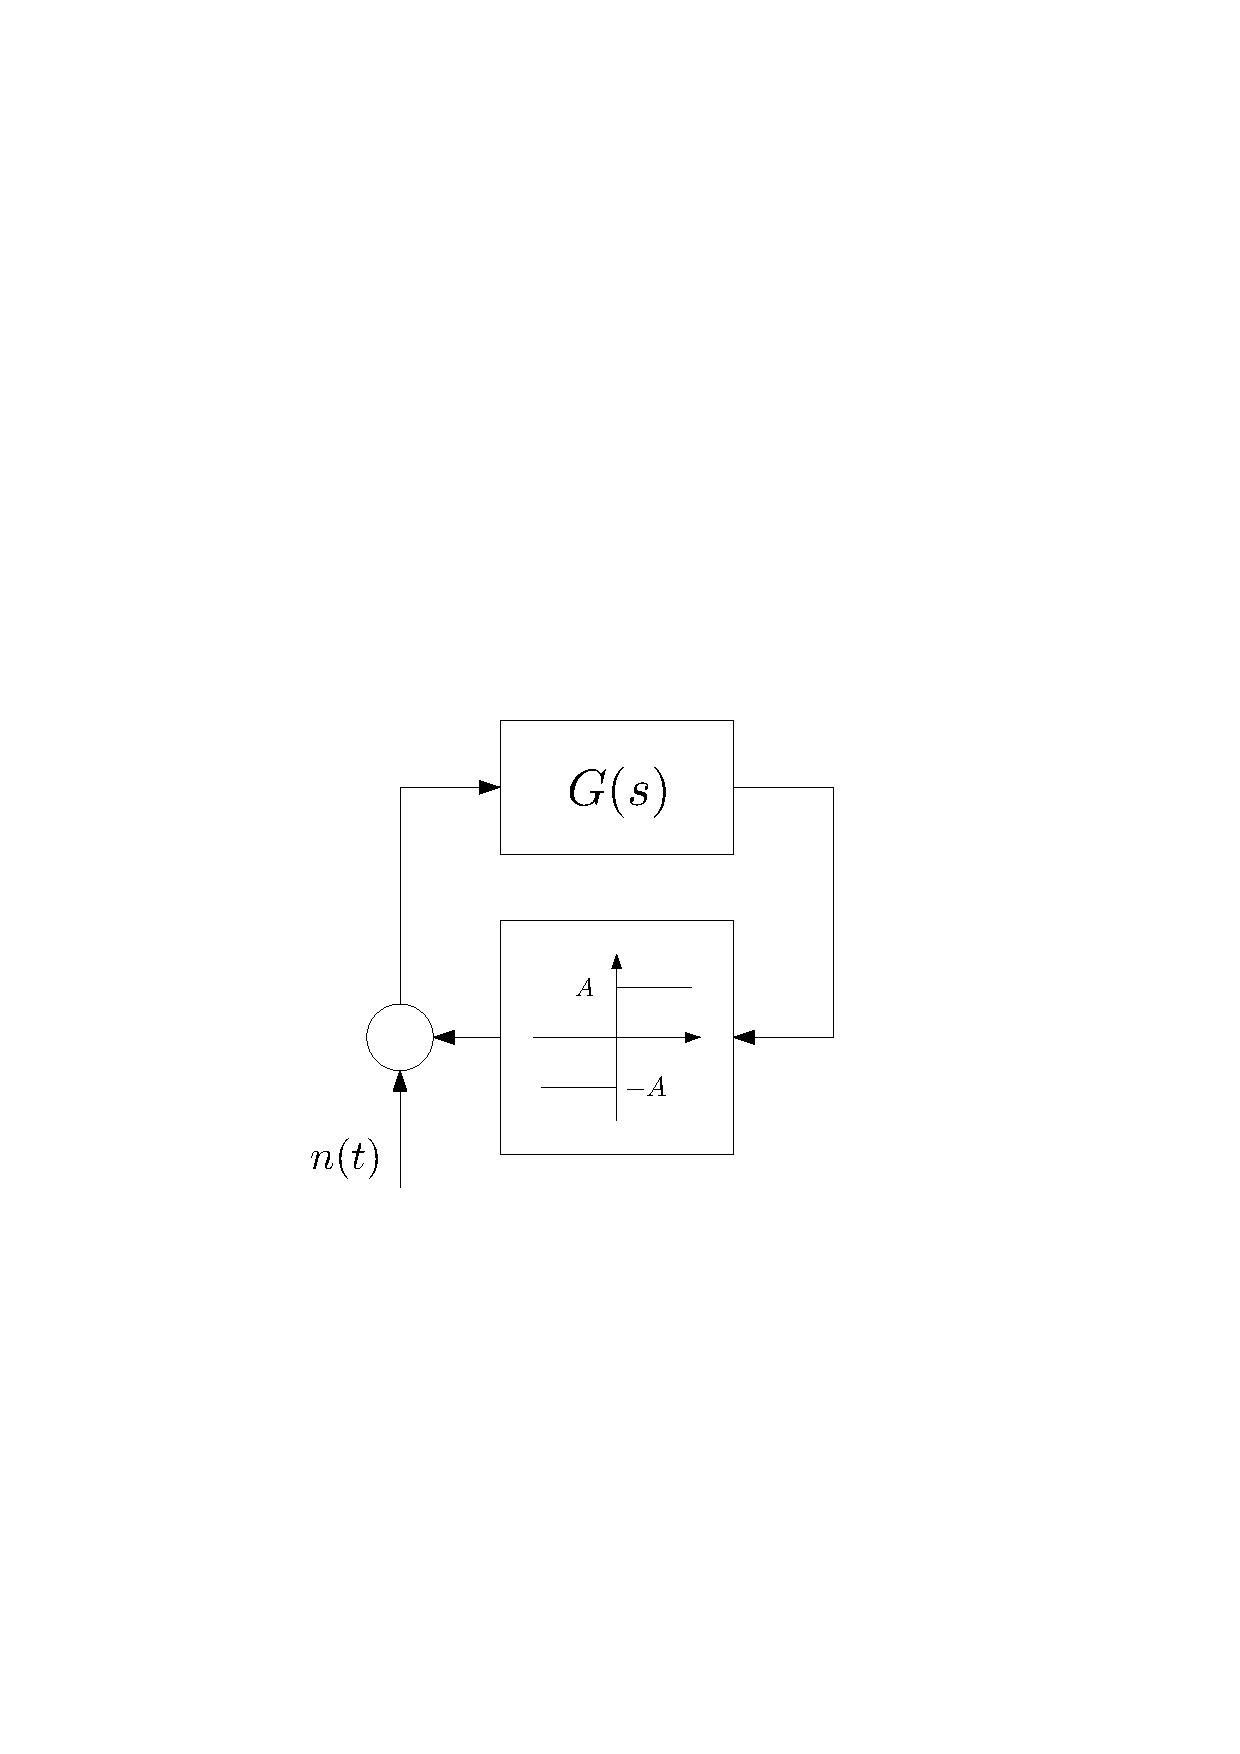
\includegraphics[width=0.5\columnwidth]{ex1scheme}
	\caption{Block diagram of the system in \ref{ex:boundednoise} \label{fig:ex1scheme}}
\end{figure}
Assume that there is an equilibrium point in the origin, that is $n(t,0)=0$,
and that we want to obtain the (practical) stabilization of the system.
% A qualitative representation of the disturbance $n(t,y)$ is provided by the gray area in the plot of Figure \ref{fig:ex1nonlin}.
% \begin{figure}
% 	\centering
% 	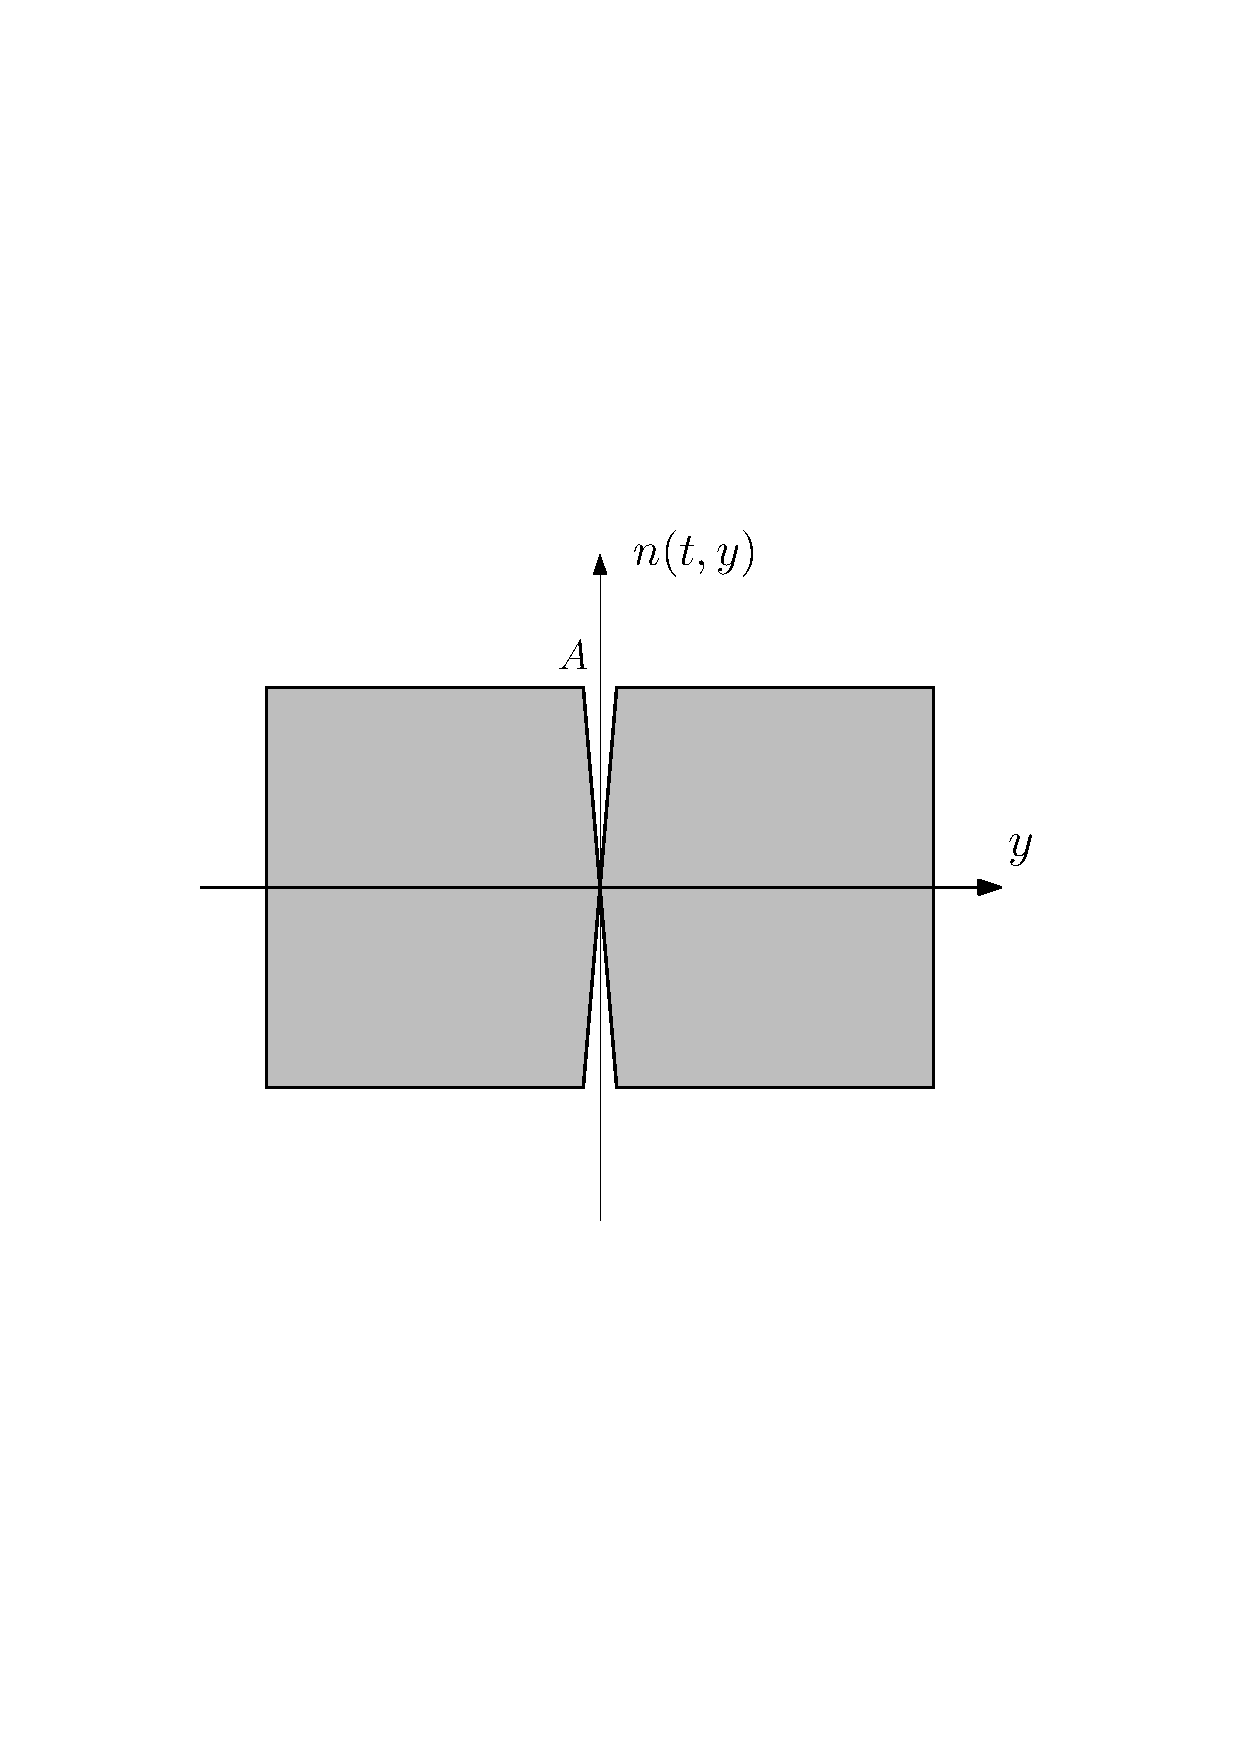
\includegraphics[width=0.75\columnwidth]{ex1nonlin}
% 	\caption{The gray area qualitatively represents the values the disturbance $n(t,y)$ can assume\label{fig:ex1nonlin}}
% \end{figure}
According to the formulation of the previous sections, we can consider both the controller and the noise together as the feedback nonlinear operator of a Lur'e system
\begin{equation*}
	\Xi(y,t)=A~\sgn(ky)+n(t,y).
\end{equation*}
Let us define $\gamma$ as the ratio between the noise bound and the controller amplitude
\begin{equation*}
	\gamma=\frac{N}{A}.
\end{equation*}
Since $A$ is a design parameter, suppose also that $0\leq~\gamma~\leq~1$.
This assumption puts the nonlinearity $\Xi(y,t)$ in the sector $[0,+\infty]$.
From the Nyquist plot of $G(s)$ depicted in Figure~\ref{fig:nyquist_quasi-posreal} it can be concluded that $G(s)$ is not positive real, so the standard Circle Criterion can not determine the stability of the system.
\begin{figure}
	\centering
	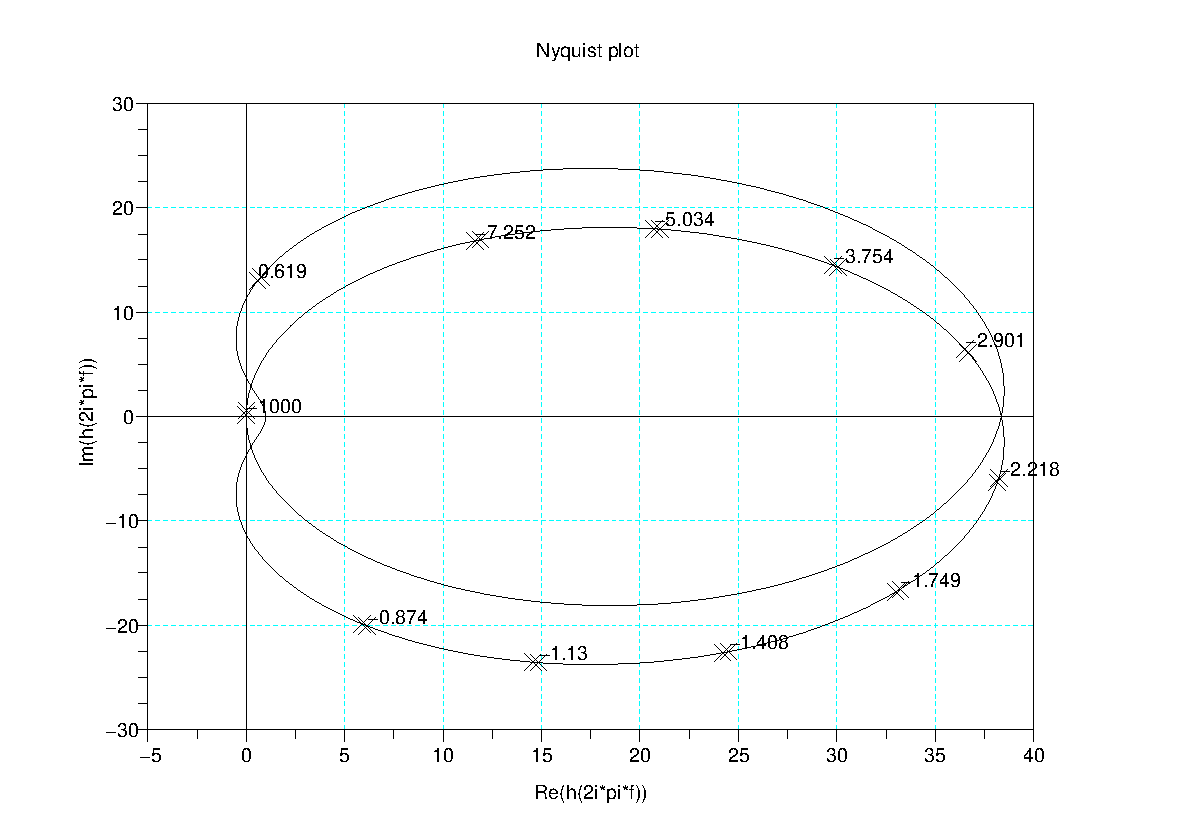
\includegraphics[width=1\columnwidth]{nyquist_quasiposreal}
	\caption{Nyquist plot of tranfer function (\ref{eq:TF_ex01}) in Example \ref{ex:boundednoise}
	\label{fig:nyquist_quasi-posreal}}
\end{figure}
The Popov and the Narendra Criteria \cite{ChoNar68} only hold for time-invariant nonlinearities, so they are not appliable.
At the same time it is not trivial to find a standard IQC satisfied by the nonlinearity
which is time-varying, non-monotonic and spanning a large sector.
We will show that it is possible to design the parameter $A$ of the feedback
controller in order to obtain a complete rejection of the noise $n(t)$.

The nonlinearity $\Xi(y,t)$ satisfies the static BIQC defined by
\begin{equation*}
	\Sigma_1=\frac{1}{\beta_1-\alpha_1}
		\left[\begin{array}{cc}
			-\alpha_1 \beta_1	& -(\alpha_1+\beta_1)\\
			-(\alpha_1+\beta_1)	& 1
		      \end{array}
		\right]
\end{equation*}
where $\alpha_1=0$, $\beta_1=0.1$ and
\begin{align*}
	M_1=\frac{1}{\beta-\alpha}(1+\gamma)^2~A ^2=10(1+\gamma)^2~A^2.
\end{align*}
Exploiting Theorem \ref{thm:2step-bottle} and solving the related LMI problem, we find that
\begin{equation*}
	\bar Y_1 =  \sqrt{M_1 \frac{CP_1^{-1}C^T}{r_1}}\leq 54.03 (1+\gamma)A,
\end{equation*}
and we conclude that, eventually, the system has a bounded output
\begin{equation*}
	|y|\leq \bar Y_1 \leq 54.03 (1+\gamma)A.
\end{equation*}
Thus, the nonlinearity will be eventually explored in a reduced sector, namely 
$\left[\frac{(1-\gamma)}{54.03(1+\gamma)}, +\infty\right)$.
If the circle corresponding to the sector
$\left[\frac{(1-\gamma)}{54.03(1+\gamma)}, +\infty\right)$
does not intersects the Nyquist plot of $G$, we can apply the standard circle criterion
and conclude global asymptotic stability for the system.
This is the case for $\gamma\leq 0.15$, as it can be confirmed by checking the feasibility
of the standard Circle Criterion in the LMI formulation. Therefore, choosing
\begin{equation}
	A>\frac{N}{0.15}
\end{equation}
we have complete rejection of the disturbance.
Furthermore suppose that the interest is in $\gamma=0.2$ ($N$ is considered fixed and therefore $A$ is smaller).
In the case $\gamma=0.2$, following the same approach, choosing
\begin{align*}
	\alpha_2=\frac{(1-\gamma)}{54.03(1+\gamma)};
	& \quad \beta_2=0.18;
\end{align*}
\begin{align*}
	M_2=\frac{1}{\beta_2-\alpha_2}(1+\gamma)^2~A ^2
\end{align*}
and solving another LMI problem, we furtherly reduce the bound of the signal $y$ to
\begin{equation*}
	\bar Y_2 =  \sqrt{M_2 \frac{CP_2^{-1}C^T}{r_2}}\leq 48.5(1+\gamma)A
\end{equation*}
which is a small reduction, but sufficient to apply the standard Circle Criterion
to the sector $\left[\frac{(1-\gamma)}{48.5(1+\gamma)}, +\infty \right)$
and conclude absolute stability also for $\gamma\leq 0.2$.
The procedure can be applied again trying to obtain global asymptotic stability
for even larger values of $\gamma$.

% DO NOT EVER DELETE THIS COMMENTS
% \subsubsection{Scilab}
% \textbf{Step 1}\\
% Use the following values:
% \begin{align}
% 	\alpha_1=0;\\
% 	\beta_1=0.1;\\
% 	M_1=\frac{1}{\beta-\alpha}(1+\gamma)^2~A ^2=10(1+\gamma)^2~A^2
% \end{align}
% So the $\Sigma$ defining the BIQC is 
% \begin{equation}
% 	\Sigma_1=\frac{1}{\beta_1-\alpha_1}
% 		\left[\begin{array}{cc}
% 			-\alpha_1*\beta_1	& -(\alpha_1+\beta_1)\\
% 			-(\alpha_1+\beta_1)	& 1
% 		      \end{array}
% 		\right]
% \end{equation}
% Remember that the sign on the entries $(1,2)$ and $(2,1)$ is given by the fact
% we are considering a positive feedback in our theoretical framework.
% Solving the related LMI problem with $r_1=2.88$, we find numerically
% \begin{equation}
% 	\bar Y_1 =  \sqrt{M_1 \frac{CP_1^{-1}C^T}{r_1}}\leq 54.03 (1+\gamma)A
% \end{equation}
% \textbf{Step 2}\\
% Now we know that eventually the system has a bounded output:
% \begin{equation}
% 	|y|\leq Y_1 \leq 54.03 (1+\gamma)A,
% \end{equation}
% so the nonlinearity is explored in a reduced sector, namely 
% $\left[\frac{(1-\gamma)}{54.03(1+\gamma)}, +\infty\right)$.
% If the circle corresponding to the sector
% $\left[\frac{(1-\gamma)}{54.03(1+\gamma)}, +\infty\right)$
% does not intersects the Nyquist plot of $G$, we can apply the standard circle criterion
% and conclude global asymptotical stability for the system.
% This is the case for $\gamma\leq 0.15$, as it can be confirmed by checking the feasibility
% of the standard Circle Criterion in the LMI formulation. So, choosing
% \begin{equation}
% 	A>\frac{N}{0.15}
% \end{equation}
% we have rejection of the disturbance.
% Let us pretend that, for the purposes of considered the application,
% the value of $A$ is still too large.
% So we want to consider if it is possible to have stability also for $\gamma=0.2$
% ($N$ is considerd fixed).
% We can perform another step using the generalized Circle Criterion.
% In the case $\gamma=0.2$, choosing
% \begin{align}
% 	\alpha_2=\frac{(1-\gamma)}{54.03(1+\gamma)};\\
% 	\beta_2=0.18;\\
% 	M_2=\frac{1}{\beta_2-\alpha_2}(1+\gamma)^2~A ^2
% \end{align}
% we actually reduce the bound of the signal $y$.
% We obtain a new bound, with $r_2=2.125$, 
% \begin{equation}
% 	\bar Y_2 =  \sqrt{M_2 \frac{CP_2^{-1}C^T}{r_2}}\leq 48.5(1+\gamma)A
% \end{equation}
% which is a small reduction, but sufficient to apply the standard Circle Criterion
% to the sector $\left[\frac{(1-\gamma)}{48.5(1+\gamma)}, +\infty \right)$
% and conclude absolute stability also for $\gamma\leq 0.2$.
% The procedure can be applied again trying to obtain global asymptotical stability
% for larger values of $\gamma$.

\subsection{Saturation with relative uncertainty}\label{subsec:ex02}
Consider the linear system $G(s)$ which was analyzed also in \cite{MegRan97}
\begin{equation}\label{eq:TF_ex02}
	G(s)=\frac{s^2}
		{s^3+2s^2+2s+1}.
\end{equation}
Its Nyquist plot is shown in Figure \ref{fig:nyquist Megretski example}.
\begin{figure}
	\centering
	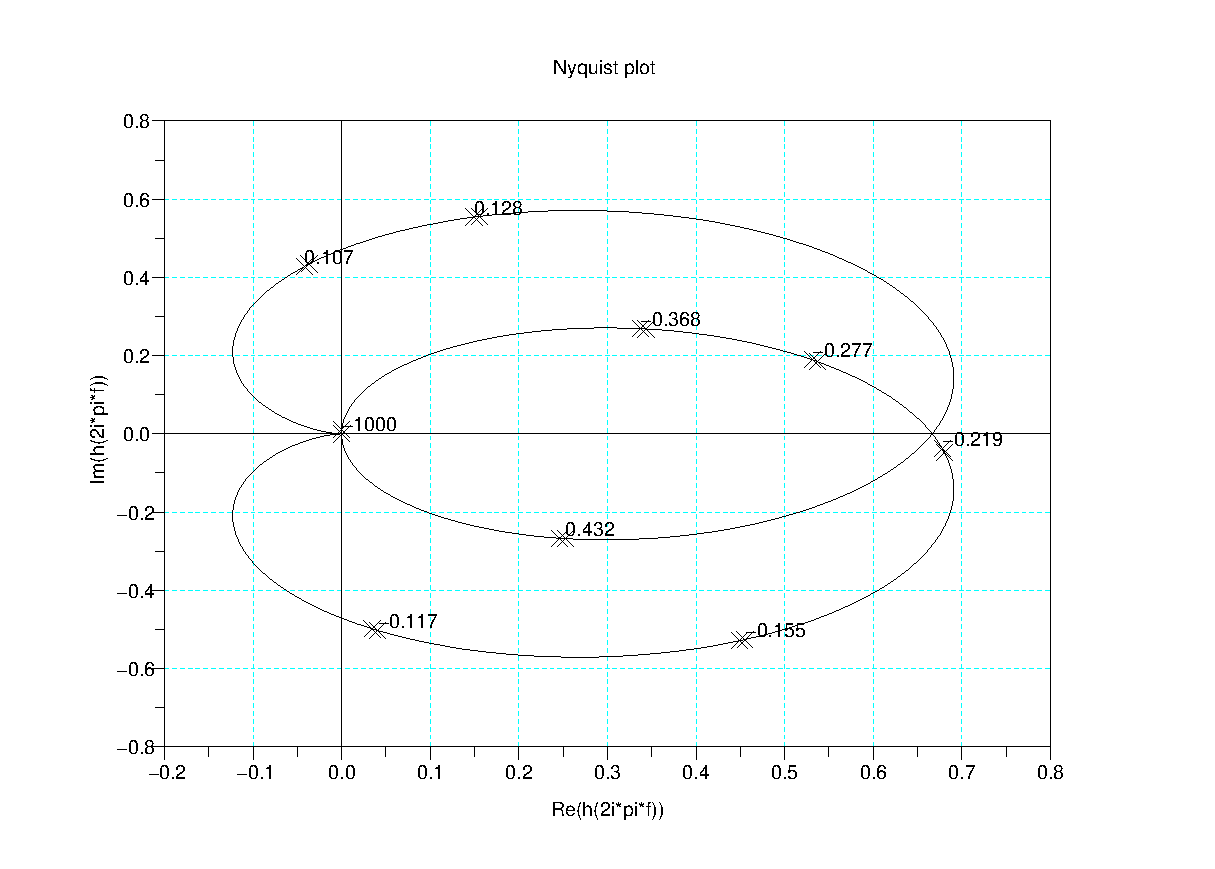
\includegraphics[width=1\columnwidth]{nyquist_MegreskiExample}
	\caption{Nyquist plot of the transfer function (\ref{eq:TF_ex02}) in example
	\ref{subsec:ex02} \label{fig:nyquist Megretski example}}
\end{figure}
We consider the transfer function $G(S)$ in feedback connection with the nonlinearity \begin{equation*}
	\Xi(y)=(1+\delta(y))\sat_A(ky)
\end{equation*}
where $\sat_A(z):=\sgn(z)\min\{|z|,A \}$ is the saturation function
% \begin{equation}
% 	\sat_A(z)=
% 		\left\{\begin{array}{ll}
% 			z & \quad \text{if}~|z|<A\\
% 			A & \quad \text{otherwise}
% 		\end{array}\right.
% \end{equation}
and $\delta(y)$ is a bounded relative uncertainty $|\delta(y)|\leq D\leq 1$ on the feedback output.
This scenario is more general than the scenario provided in \cite{MegRan97} where there is no uncertainty ($D=0$).
We want to study how the parameter $k$ influences the stability of the system.
It immediately follows that the nonlinearity $\Xi(\cdot)$ is in the sector $[0, k(1+D)]$. The application of the Circle Criterion provides a conservative result stating that the system is stable for $k(1+D)< k_{cc}\simeq 8.13$.
The Popov criterion improves the result by a small amount, guaranteeing stability for $k(1+D)< k_{pc}\simeq 8.90$.
When there is no uncertainty ($D=0$), it would possible to exploit a powerful result by Zames and Falb for monotonic and odd nonlinearities which guarantees stability for any positive value of $k$. Indeed, it can be shown that monotonic and odd nonlinearities satisfy the IQC
\begin{equation*}
	\int_{-\infty}^{+\infty}
		\left(\begin{array}{c}
			\hat y(t) \\
			\hat \csi(t)
		\end{array}\right)^*
		\left(\begin{array}{cc}
			0 		& 1+\hat h(i\w)\\
			1+\hat h(-i\w)	& -2(1+ \text{Re}\{\hat h(i\w)\})/k
		\end{array}\right)
		\left(\begin{array}{c}
			\hat y(t) \\
			\hat \csi(t)
		\end{array}\right)
	dt \geq 0
\end{equation*}
where $H(s)$ is any transfer function such that its $l_1$ norm is less or equal than~$1$.
In the uncertain case, such a result can not be used at least in the standard form.
However, as in Lemma \ref{lem:from dynamic 2 static IQC}, we can consider the standard associated IQC formulated in the time domain
\begin{align*}
	\int_{0}^{+\infty}[ky(t)-\csi(t)][\csi(t)+h(t)*\csi(t)]\geq 0
% 		\qquad \geq -A^2D^2(1+\|h\|_1) dt \geq 0
\end{align*}
and note that in our case
\begin{align*}
	[ky(t)-\csi(t)][\csi(t)+h(t)*\csi(t)] +A^2D^2(1+\|h\|_1) \geq 0.
\end{align*}
Therefore, even though the standard Zames-Falb IQC is not satisfied, the associated time-domain BIQC is met
\begin{equation*}
	\limsup_{t\rightarrow +\infty}
	\int_{0}^{t}
		\left[
		\left(\begin{array}{c}
			\hat y_\pi(\tau) \\
			\hat y(\tau) \\
			\hat \csi(\tau)
		\end{array}\right)^*
		\left(\begin{array}{ccc}
			0	& k	& -1\\
			k	& 0	& k \\
			-1	& k	& -2
		\end{array}\right)
		\left(\begin{array}{c}
			\hat y_\pi(\tau) \\
			\hat y(\tau) \\
			\hat \csi(t)
		\end{array}\right)
		+ M
		\right]
	d\tau \geq 0
\end{equation*}
with $\hat y_{\pi}=H(i\w)\hat \csi$ and $M>2A^2D^2(1+\|h\|_1)$.
Suppose, as in \cite{MegRan97}, that $H(i\w)=-1/(1+i\w)$,
while the objective is to find a maximum value of $k$ providing the stability of the system as a function of the uncertainty parameter $D$.
Applying Theorem~\ref{thm:EPI set for lur'e systems} we find that eventually the output $y(t)$ will be bounded
\begin{equation*}
	|y(t)|< \overline Y := A D \sqrt{\frac{CP^{-1}C^T}{r}}.
\end{equation*}
Therefore, the nonlinearity will be explored in the interval $[-\bar Y, \bar Y]$, making it possible to consider just the sector $[ A(1-D)/\bar Y , k(1+D)]$.
Given $D$, the maximum value for $k$ which provides stability can be found in a second step by applying the Popov or the Circle criterion.
Results for different values of the uncertainty parameter $D$ are provided in Figure~\ref{fig:maxkversusD}.
\begin{figure}
	\centering
	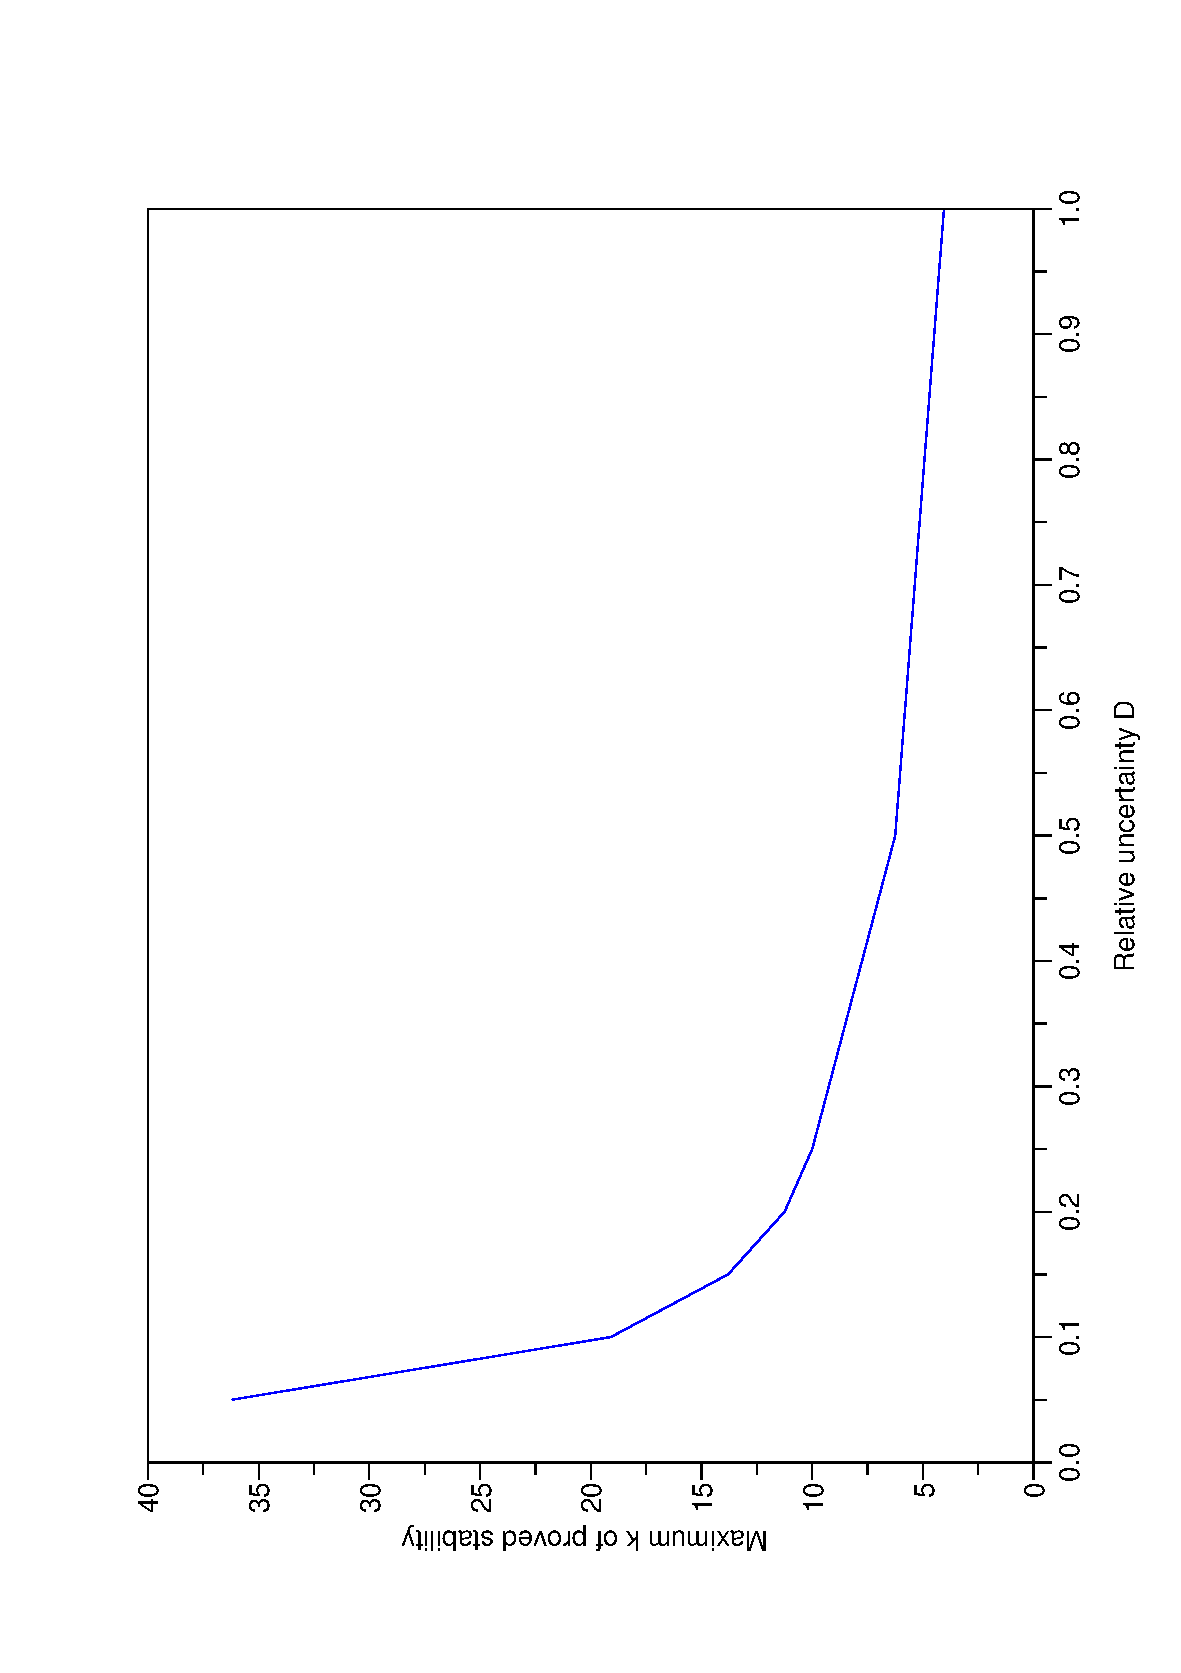
\includegraphics[width=0.75\columnwidth, angle=-90]{MaxKversusD}
	\caption{Maximum $k$ of proved stability versus D
		\label{fig:maxkversusD}}
\end{figure}
When $D$ is close to zero we find that the gain $k$ can be very large and can still provide global asymptotic stability of the system. Conversely, when $D$ increases the interval of values for which $k$ provides guaranteed stability shrinks.

% DO NOT EVER DELETE THIS COMMENTS
% Consider the linear system $G(s)$ analyzed also in \cite{MegRan97}
% \begin{equation}
% 	G(s)=\frac{s^2}
% 		{s^3+2s^2+2s+1}
% \end{equation}
% The Nyquist plot of $G(s)$ is reported in Figure \ref{fig:nyquist Megretski example}.
% \begin{figure}
% 	\centering
% 	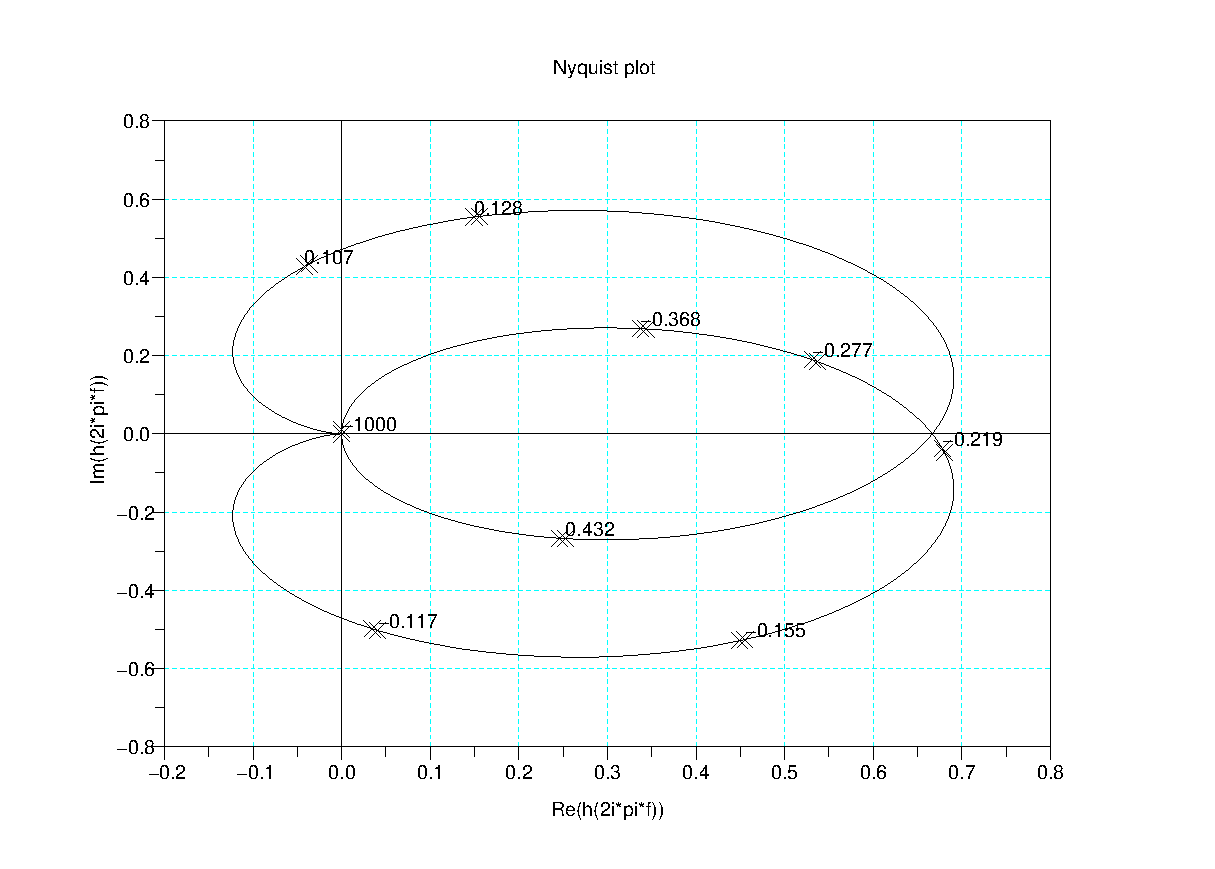
\includegraphics[width=1\columnwidth]{nyquist_MegreskiExample}
% 	\caption{Hello, I am a Nyquist plot\label{fig:nyquist Megretski example}}
% \end{figure}
% The transfer function $G(S)$ is fedback by the nonlinearity $\Xi(t,y)$
% \begin{equation}
% 	\Xi(y)=(1+\delta(y))\sat_A(ky)
% \end{equation}
% where 
% \begin{equation}
% 	\sat_A(z)=
% 		\left\{\begin{array}{ll}
% 			z & \quad \text{if}~|z|<A\\
% 			A & \quad \text{otherwise}
% 		\end{array}\right.
% \end{equation}
% and $\delta(y)$ is a bounded relative uncertainty
% \begin{equation}
% 	|\delta(y)|\leq D\leq 1
% \end{equation}
% on the feedback output. We want to study how the parameter $k$ influences the stability of the system. It is immediate to note that the nonlinearity $\Xi(\cdot)$ is in the sector $[0, k(1+D)]$. The application of the Circle Criterion provides a conservative result stating that the system is stable for
% \begin{equation}
% 	k(1+D)< k_{cc}\simeq 8.13
% \end{equation}
% The Popov criterion improves the result by a small amount, guaranteeing stability for
% \begin{equation}
% 	k(1+D)< k_{pc}\simeq 8.90
% \end{equation}
% When there is no uncertainty ($D=0$), it would possible to exploit a powerful result by Zames and Falb for monotonic and odd nonlinearities which guarantees stability for any positive value of $k$. In the uncertain case, such a result can not be used at least
% in the standard form.
% Consider a transfer function $H(s)$ such that its pulse response $h(\tau)$ has $1$-norm lesser than $1$. We note that
% \begin{align}
% 	[ky(t)-\csi(t)][\csi(t)+h(t)*\csi(t)]\geq \\
% 		\qquad \geq -A^2D^2(1+\|h\|_1)
% \end{align}
% So, even though the standard Zames-Falb IQC in the frequency domain
% \begin{equation}
% 	\int_{-\infty}^{+\infty}
% 		\left(\begin{array}{c}
% 			\hat y(t) \\
% 			\hat \csi(t)
% 		\end{array}\right)^*
% 		\left(\begin{array}{cc}
% 			0 		& 1+H(i\w)\\
% 			1+H(-i\w)	& -2(1+ \text{Re}\{H(i\w)\})/k
% 		\end{array}\right)
% 		\left(\begin{array}{c}
% 			\hat y(t) \\
% 			\hat \csi(t)
% 		\end{array}\right)
% 	dt \geq 0
% \end{equation}
% is not satisfied, the associated time-domain BIQC is met
% \begin{equation}
% 	\limsup_{t\rightarrow +\infty}
% 	\int_{0}^{t}
% 		\left[
% 		\left(\begin{array}{c}
% 			\hat y_\pi(\tau) \\
% 			\hat y(\tau) \\
% 			\hat \csi(\tau)
% 		\end{array}\right)^*
% 		\left(\begin{array}{ccc}
% 			0	& k	& -1\\
% 			k	& 0	& k \\
% 			-1	& k	& -2
% 		\end{array}\right)
% 		\left(\begin{array}{c}
% 			\hat y_\pi(\tau) \\
% 			\hat y(\tau) \\
% 			\hat \csi(t)
% 		\end{array}\right)
% 		+ M
% 		\right]
% 	d\tau \geq 0
% \end{equation}
% with $\hat y_{\pi}=H(i\w)\hat \csi$ and $M>2A^2D^2(1+\|h\|_1)$.
% Let us choose
% \begin{align}
% 	H(i\w)=-\frac{1}{1+i\w}
% \end{align}
% and let us find a maximum value of $k$ providing the stability of the system as a function of the uncertainty parameter $D$.
% Applying Theorem \ref{thm:EPI set for lur'e systems} we find that eventually the output $y(t)$ will be bounded
% \begin{equation}
% 	|y(t)|< \bar Y := A D \sqrt{\frac{CP^{-1}C^T}{r}}
% \end{equation}
% So, the nonlinearity will be explored in the interval $[-\bar Y, \bar Y]$, making it possible to consider it spanning just the sector $[ A(1-D)/\bar Y , k(1+D)]$.
% Given $D$, the maximum value for $k$ which provides stability can be found by applying the Popov or the Circle criterion.
% Results are provided in Figure \ref{fig:maxkversusD}.
% \begin{figure}
% 	\centering
% 	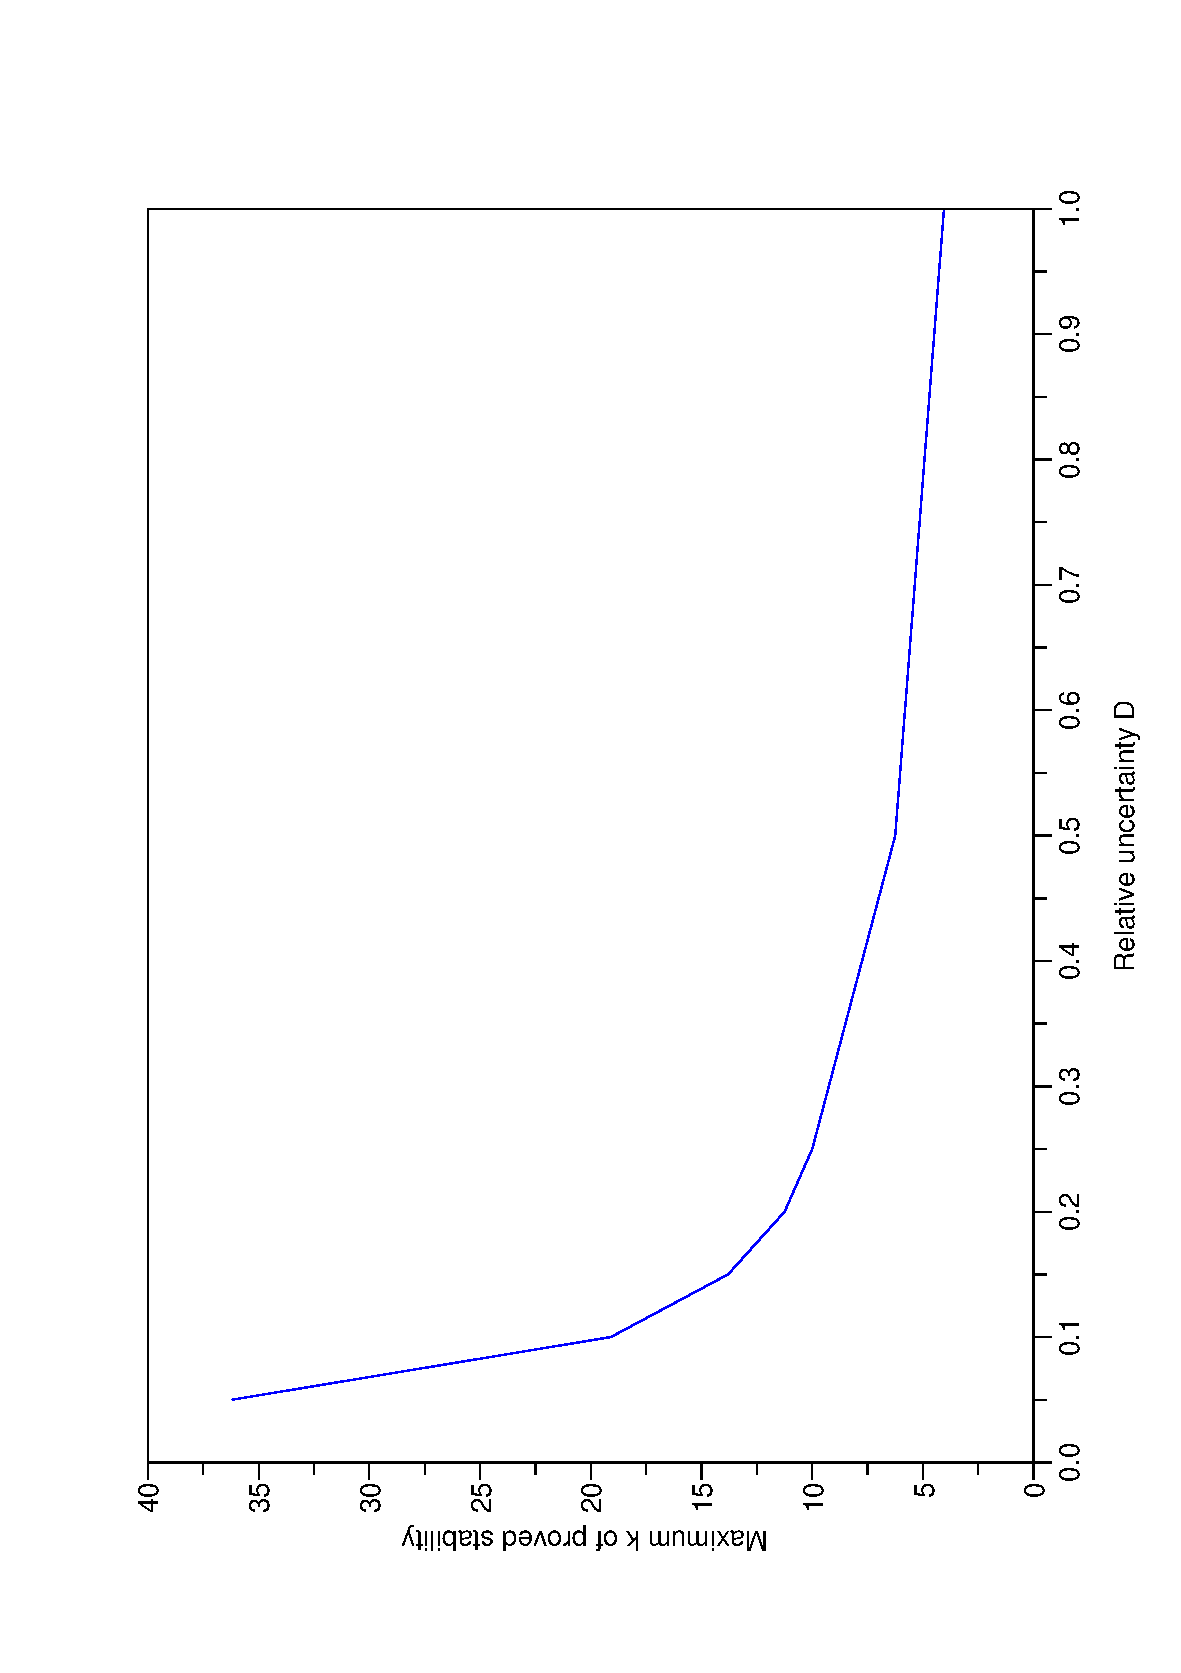
\includegraphics[width=0.75\columnwidth, angle=-90]{MaxKversusD}
% 	\caption{Maximum $k$ of proved stability versus D
% 		\label{fig:maxkversusD}}
% \end{figure}

\section{Conclusion}
In this paper we have introduced the concept of Biased Integral Quadratic Constraint and we have derived results to conclude eventual global boundedness of the system trajectories.
This notion is also known in literature as practical stability. Further it is shown how to exploit the bound information in order to prove asymptotic stability.
Indeed, the boundedness property allows one to consider the nonlinearity to be explored in a smaller region (after a finite time). Stricter BIQC's can be then exploited to obtain a better bound or to conclude the stability of the system.

\begin{appendix}

\subsection{Proof of Lemma \ref{lem:lyapliminf}}
	Given $\eps>0$, suppose there exists $t_2$ such that $t>t_2$ implies that $V(t)\geq \frac{M}{r}+\eps$.
	Since $\sigma(t)+M$ has non-negative liminf integral,
	there exists $t_1$ such that for $t>t_1$
	\begin{equation*}
		\int_0^{~t}[\sigma(\tau)+M]d\tau\geq -\eps.
	\end{equation*}
	Integrating both sides of (\ref{eq:diffV_lem_liminf}) with $t>\max(t_1,t_2)$
	\begin{equation*}
		0\leq V(t)< V(0)-r\int_{0}^{t}V(\tau)d\tau+Mt+\eps<V(0)-r\eps~t+\eps.
	\end{equation*}
	Choosing $t>(V(0)+\eps)/(r\eps)$ we have a contradiction.

\subsection{Proof of Lemma \ref{lem:conv_sigma^(-)}}
	Since the Lebesgue integral exists, at least one of the two integrals
	\begin{equation*}
		\int_0^{+\infty}\gamma^{(-)}(\tau)d\tau,
			\qquad
		\int_0^{+\infty}\gamma^{(+)}(\tau)d\tau
	\end{equation*}
	is finite. Also the integrals
	\begin{equation*}
		\int_0^{t}\gamma^{(-)}(\tau)d\tau,
			\qquad
		\int_0^{t}\gamma^{(+)}(\tau)d\tau
	\end{equation*}
	are finite for all $t\geq 0$.
	By (\ref{eq:liminfpositive}), given $\eps>0$,
	there exists $T_{\eps}$ such that $t>T_{\eps}$ implies
	\begin{equation*}
% 		\inf_{t>T} 
			\int_0^{t}\gamma(\tau)d\tau>\alpha-\eps.
	\end{equation*}
	With $\eps=\alpha/2$, we have that
% 	\begin{equation}
% 		\inf_{t>T} \int_0^{t}\gamma(\tau)d\tau>\frac{\alpha}{2}>0
% 	\end{equation}
% 	Thus
	\begin{equation*}
		\int_0^{t}\gamma^{(+)}(\tau)d\tau>
			\int_0^{t}\gamma^{(-)}(\tau)d\tau+\frac{\alpha}{2}.
	\end{equation*}
	If
	\begin{equation*}
		\lim_{t\rightarrow +\infty}\int_0^{t}\gamma^{(-)}(\tau)d\tau=+\infty
	\end{equation*}
	we clearly have a contradiction of the hypothesis.

\subsection{Proof of Lemma \ref{lem:Vlimsupbounded}}
	Fix $\eps>0$ and define $\gamma(t):=\sigma(t)+M$.
	By Lemma \ref{lem:conv_sigma^(-)}, we have that
	\begin{equation*}
		\lim_{t\rightarrow +\infty}
			\int_0^{t}\gamma^{(-)}(\tau)d\tau<+\infty.
	\end{equation*}
	Thus, by the theorem of Cauchy sequence, it is always possible to find $T_1$
	such that $T_1<t_a\leq t_b$ implies
	\begin{equation*}
		\int_{t_a}^{t_b}\gamma^{(-)}(\tau)d\tau>-\eps/2.
	\end{equation*}
	It follows from Lemma \ref{lem:lyapliminf}, that there exists a $t_0>T_1$ such that $V(t_0)<\frac{M}{r}+\eps$. We now want to prove that $t>t_0$ implies $V(t)<\frac{M}{r}+\eps$. By contradiction suppose there exists $t_2$ such that $t_2>t_0$ and $V(t_2)\geq\frac{M}{r}+\eps$.
	Because of the continuity of $V(x(\cdot))$ there must exist
	$t_1$ such that $t_0<t_1<t_2$, $V(t_1)=\frac{M}{r}+\eps/2$
	and $V(t)\geq \frac{M}{r}+\eps/2$ for $t_1\leq t \leq t_2$.
	Integrating (\ref{eq:diffV_lem_lim}) from $t_1$ to $t_2$
	\begin{align*}
		V(t_2)	&<V(t_1)-r\int_{t_1}^{t_2}V(t)d\tau
				+M(t_2-t_1) -\int_{t_1}^{t_2}\gamma(\tau)d\tau <\\
			&<\frac{M}{r}+\frac{\eps}{2}
				-r\int_{t_1}^{t_2}\left[V(t)-\frac{M}{r}\right]d\tau
				-\int_{t_1}^{t_2}\gamma^{(+)}(\tau)d\tau +\\
				&\qquad+\int_{t_1}^{t_2}\gamma^{(-)}(\tau)d\tau
			\leq\frac{M}{r}+\frac{\eps}{2}+\frac{\eps}{2}=\frac{M}{r}+\eps
	\end{align*}
	which leads to a contradiction. This proves the lemma.

% \begin{lem}
% 	Let $\Pi(s)\in\mathcal{C}^{(p+m)\times(p+m)}$ be real rational and globally bounded on the imaginary axis $s=i\w$ with $\w\in\Real$ and $p,m\in \mathbb{N}$.
% 	Then, $\Pi(s)$ admits the following factorization
% 	\begin{equation}\label{eq:PIfactorization}
% 		\Pi(s)=
% 			\left(\begin{array}{cc}
% 				T_1(s)		& T_2(s)\\
% 				I_m		& 0 \\
% 				0		& I_p
% 			\end{array}\right)^*
% 			\Gamma
% 			\left(\begin{array}{cc}
% 				T_1(s)		& T_2(s)\\
% 				I_m		& 0 \\
% 				0		& I_p
% 			\end{array}\right)
% 	\end{equation}
% 	with $T(s):=(T_1(s) ~ T_2(s))$ proper, stable and minimum phase.
% \end{lem}
% \begin{proof}
% 	TODO: see \cite{}
% \end{proof}
\end{appendix}

\bibliography{abstab}
\end{document}